
%\documentclass[12pt]{report}
%\documentclass[12pt]{extreport}
\documentclass[17pt]{extarticle}

\AddToHook{cmd/section/before}{\clearpage} % a new page for each new section!!!

%\documentclass{memoir}

\usepackage{graphicx}
\usepackage{setspace}
\usepackage{amsmath,amssymb}
\usepackage{IEEEtrantools}
\usepackage{cancel}
\usepackage[font=small,labelfont=bf]{caption}


\usepackage{verbatim}

\usepackage[T1]{fontenc}
\usepackage[utf8]{inputenc}
\usepackage[italian]{babel}

\usepackage{imakeidx}
\usepackage{hyperref}
\makeindex


\usepackage{geometry}
 \geometry{
 a4paper,
 total={170mm,264mm},
 left=16mm,
 top=10mm,
 }



\newcommand{\pict}[1]{
\begin{figure}[h!]		
	\centering
   	\includegraphics[width=7.0in]{pictures/picture_#1.png}
  	\caption{#1}
   	\label{fig:LibreOfficeCalc#1}
\end{figure}
}



\begin{document}

\begin{flushright}
{\bf \today}
\end{flushright}

\tableofcontents

\clearpage


Abbiamo visto analiticamente\footnote{Cioè facendo i calcoli} che, data una equazione lineare in due incognite $x$ e $y$, una sua possibile soluzione è una \emph{coppia ordinata} di numeri. 


Ad esempio, data l'equazione 

\begin{equation}\label{eq:eqLineare}
	9y - 7x - 3 = 0
\end{equation}

attribuendo a $x$ il valore $0$, si ottiene per $y$ il valore $\frac{1}{3}$, attribuendo a $x$ il valore $1$, si ottiene per $y$ il valore $\frac{10}{9}$ e così via, come nella tabella che segue


\begin{center}
\begin{tabular}%\label{tab:eqLineare}
	{ |c|c| c| }
 \hline
 {\bf x} &  {\bf y} &  $y$ approssimato \\ 
 \hline
 0 & $\frac{1}{3}$  &  $0,33$ \\
 1 & $\frac{10}{9}$ &  $0,11$ \\ 
 2 & $\frac{17}{9}$ &  $1,89$ \\ 
 3 & $\frac{24}{9}$ &  $2,67$ \\ 
 4 & $\frac{31}{9}$ &  $3,44$ \\ 
 5 & $\frac{38}{9}$ &  $4,22$ \\ 
$\dots$ & $\dots$	& $\dots$\\	
 \hline

%\caption{Tabella delle possibile coppie ordinate di valori $x$ e $y$ soluzioni dell'equazione lineare in due incognite.}
\end{tabular}
\end{center}


%essendo \emph{infiniti} i differenti valori che posso attribuire a $x$, infiniti sono anche i possibili valori di $y$. 

Abbiamo anche visto, adoperando la carta millimetrata, che le infinite coppie ordinate che risolvono una equazione lineare come la eq. \ref{eq:eqLineare} \emph{giacciono tutte e solo} su una ben precisa retta (fig. \ref{fig:LibreOfficeCalc000}). 



\pict{000}

% Le coppie ordinate della tabella precedente, soddisfano l'equazione lineare $9y -7x - 3 = 0$ e quindi corrispondono a punti sul piano cartesiano che stanno tutti su una stessa retta.

Sempre adoperando la carta millimetrata, abbiamo visto che mettendo a sistema due differenti equazioni lineari, la coppia ordinata risultato del sistema è, graficamente, il punto di intersezione delle rispettive rette. In questa sede andiamo a rivedere tutto questo facendo uso del \emph{foglio di calcolo elettronico} e, in particolare, di LibreOffice Calc.



\section{Rappresentazione grafica di una retta su piano cartesiano con \emph{foglio di calcolo elettronico} }


%Inoltre, il risultato di un sistema due equazioni lineari e due incognite, quando ammette una unica soluzione\footnote{le soluzioni possono essere \emph{infinite} quando il sistema è indeterminato o nessuna, quando il sistema è \emph{impossibile}.}, è una \emph{coppia ordinata} di numeri che corrispondono alle coordinate del punto di intersezione tra le due rette associate a ciascuna delle due equazioni.

%Data una equazione lineare in due variabili $x$ e $y$, come ad esempio

%usiamo il foglio di calcolo elettronico e, in particolare, \emph{LibreOffice Calc}, per calcolare il valore delle coppie ordinate che soddisfano una equazione

%sono infinite
Prendiamo in considerazione il sistema due equazioni lineari e due incognite:

\begin{equation}\label{eq:sistema}
  	\begin{cases}
		9y - 2x + 12 = 0\\
		9y + 7x + 3 = 0		
	\end{cases}
\end{equation}

Facendo uso di LibreOffice Calc, per ciascuna delle equazioni di questo sistema, andiamo a calcolare una tabella, come quella del paragrafo precedente.

Per fare ciò, conviene che per ciascuna delle due equazioni del sistema \ref{eq:sistema}, esplicitiamo la $y$ in funzione della $x$


\begin{equation}\label{eq:sistemaEspl}
  	\begin{cases}
		y = \frac{2}{9}x - \frac{4}{3}\\
		y = -\frac{7}{9}x - \frac{1}{3}
	\end{cases}
\end{equation}


Passiamo ora a LibreOffice Calc (fig. \ref{fig:LibreOfficeCalc003})
%\begin{figure}[h!]		
	\centering
   	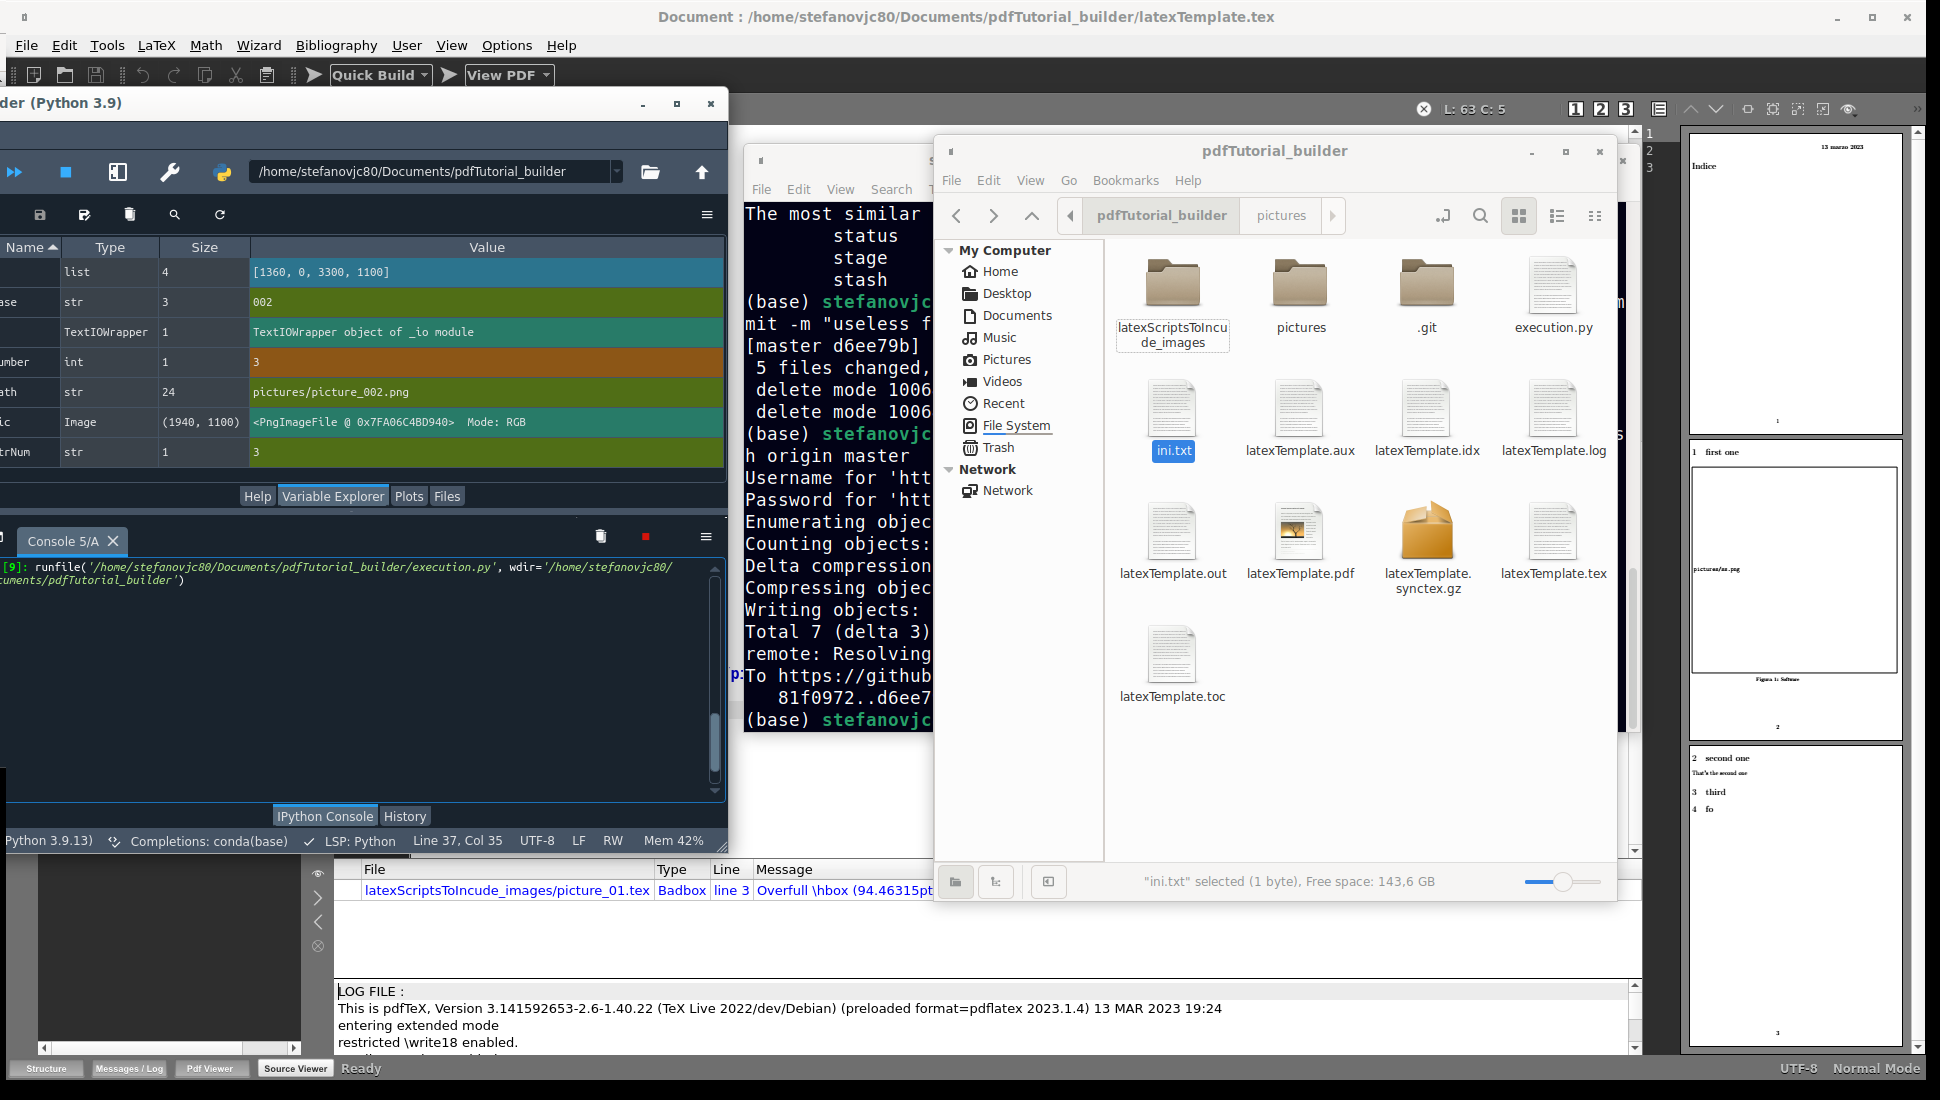
\includegraphics[width=8.0in]{pictures/picture_003.png}
  	\caption{LibreOffice Calc}
   	\label{fig:LibreOfficeCalc003}
\end{figure}


\section{Scrittura nelle caselle di testo, numeri e formule matematiche}

Con riferimento alla figura \ref{fig:LibreOfficeCalc003}, andiamo ad usare le colonne A, B e C. 

\pict{003}

La {\bf prima riga } di tutte e tre le colonne la usiamo come "titolo" alla colonna stessa; come in figura \ref{fig:LibreOfficeCalc004}. In particolare

\begin{itemize}
	\item la {\bf colonna A} per i valori delle {\bf x} che andiamo a scegliere \footnote{Selezionare la casella A1 con il mouse, scrivere "x" e premere \emph{invio}. }
	\item la {\bf colonna B} per i valori di $y$ calcolati da x con la prima equazione del sistema numero \ref{eq:sistemaEspl} (che chiamiamo {\bf y1})
	\item la {\bf colonna C} per i valori $y$ calcolati da x con la seconda equazione del sistema numero \ref{eq:sistemaEspl} (che chiamiamo {\bf y2})
\end{itemize}

\vspace{1cm}

Nella {\bf Seconda riga} 

\begin{itemize}
	\item $-10$ in A2  come primo valore di $x$.
	\item Nella casella B2 va messa la prima equazione del sistema \ref{eq:sistemaEspl}.
	\item Nella casella C2 va messa la seconda equazione del sistema \ref{eq:sistemaEspl}.
\end{itemize}

 



Iniziamo con la casella B2. Per istruire il software che in questa casella ci va una espressione algebrica da calcolare, e non semplicemente del testo, va inizializzata con il carattere "=", al quale segue l'espressione $\frac{2x}{9} - \frac{4}{3}$ (figura \ref{fig:LibreOfficeCalc005}).
%Nella casella B2 poniamo  il valore y1 calcolato in funzione del contenuto della casella A2 

%La prima equazione di \ref{eq:sistemaEspl} viene quindi inserita nella casella B2 (figura \ref{fig:LibreOfficeCalc005}).

Allo stesso modo, nella casella C2 mettiamo l'espressione algebrica corrispondente a $-\frac{7x}{9} - \frac{1}{3}$ (figura \ref{fig:LibreOfficeCalc006})



\pict{004}



%\begin{figure}[h!]		
	\centering
   	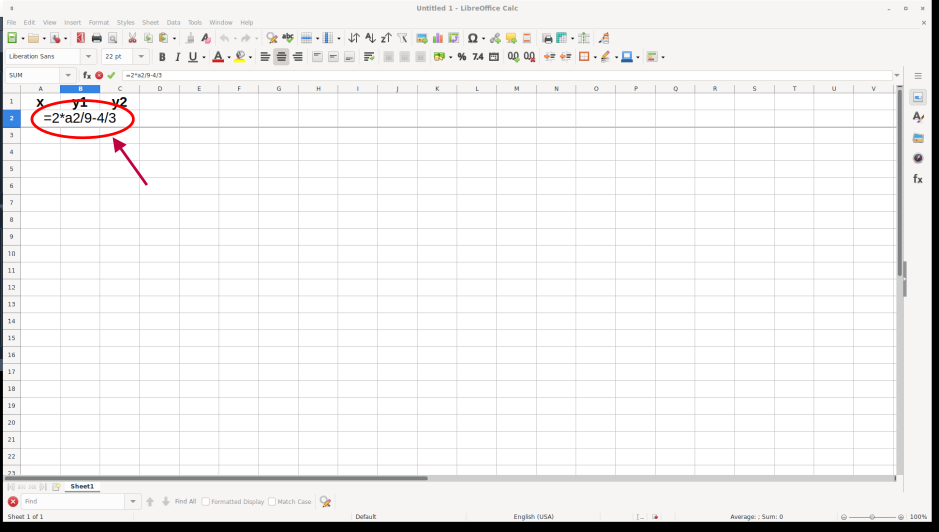
\includegraphics[width=8.0in]{pictures/picture_005.png}
  	\caption{LibreOffice Calc}
   	\label{fig:LibreOfficeCalc005}
\end{figure}
\pict{005}

%Allo stesso modo, nella casella $C2$ immattiamo il secondo membro della seconda equazione del sistema \ref{eq:eqLineare}ref{eq:sistemaEspl}

%\begin{figure}[h!]		
	\centering
   	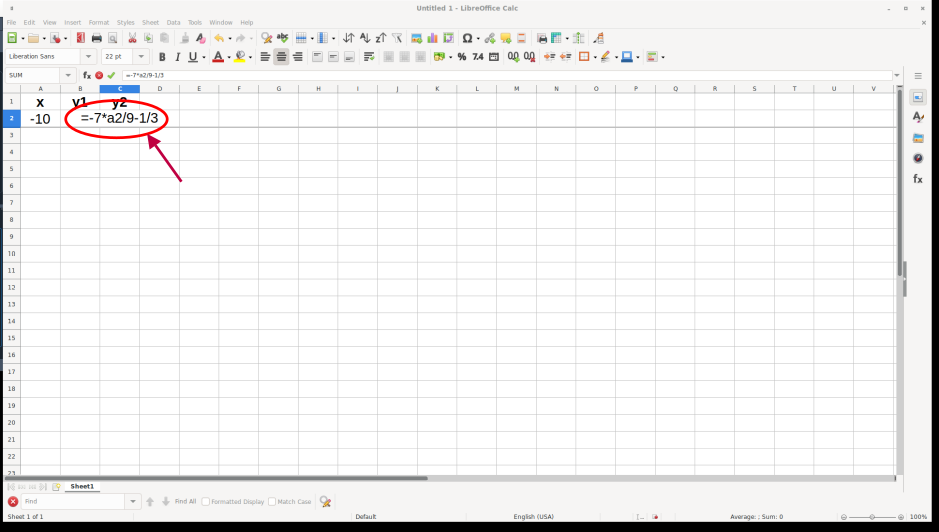
\includegraphics[width=8.0in]{pictures/picture_006.png}
  	\caption{LibreOffice Calc}
   	\label{fig:LibreOfficeCalc006}
\end{figure}
\pict{006}


Il risultato che dovrebbe apparire è riportato nella figura \ref{fig:LibreOfficeCalc007}


%\begin{figure}[h!]		
	\centering
   	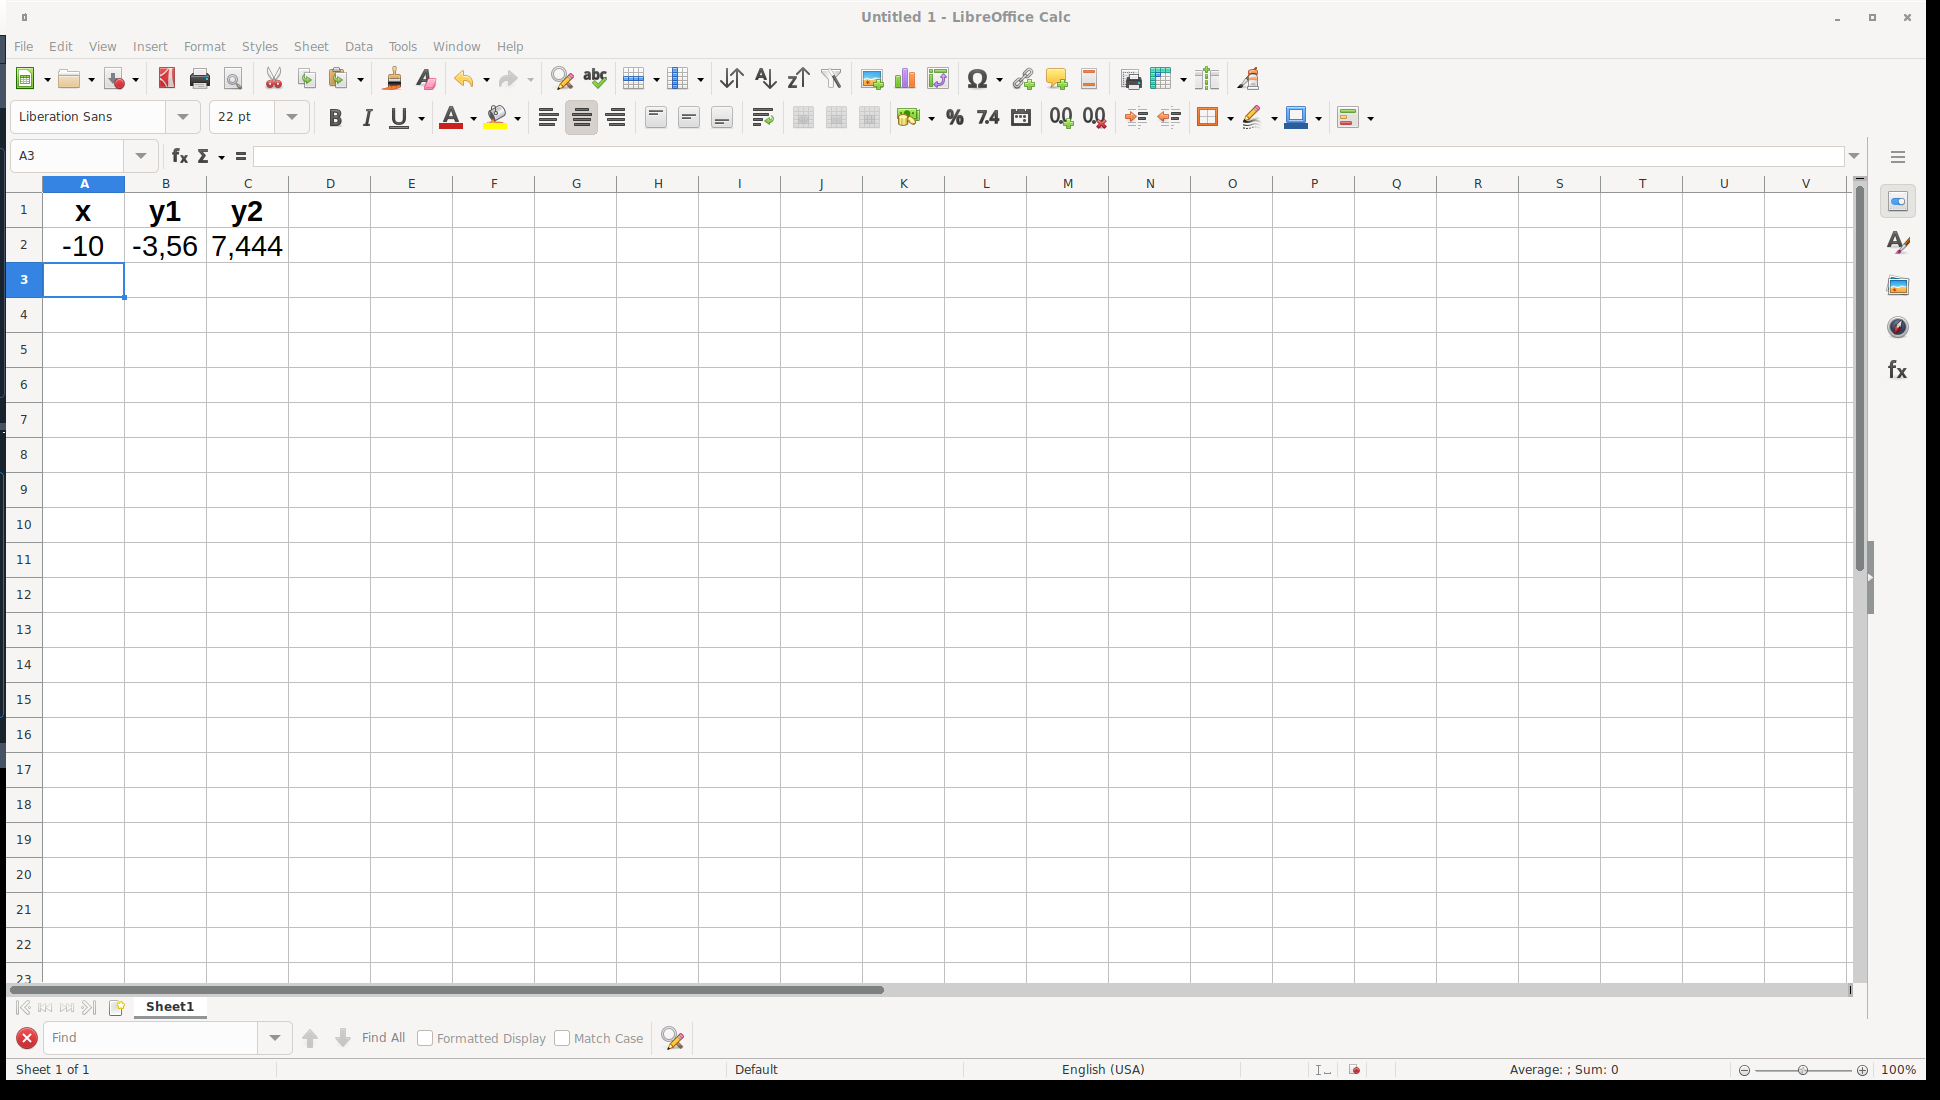
\includegraphics[width=8.0in]{pictures/picture_007.png}
  	\caption{LibreOffice Calc}
   	\label{fig:LibreOfficeCalc007}
\end{figure}
\pict{007}


\section{Copiatura delle formule matematiche su più caselle della medesima colonna}

Scriviamo ora l'espressione algebrica "$=a2 + 0,01$" nella casella A3

%\begin{figure}[h!]		
	\centering
   	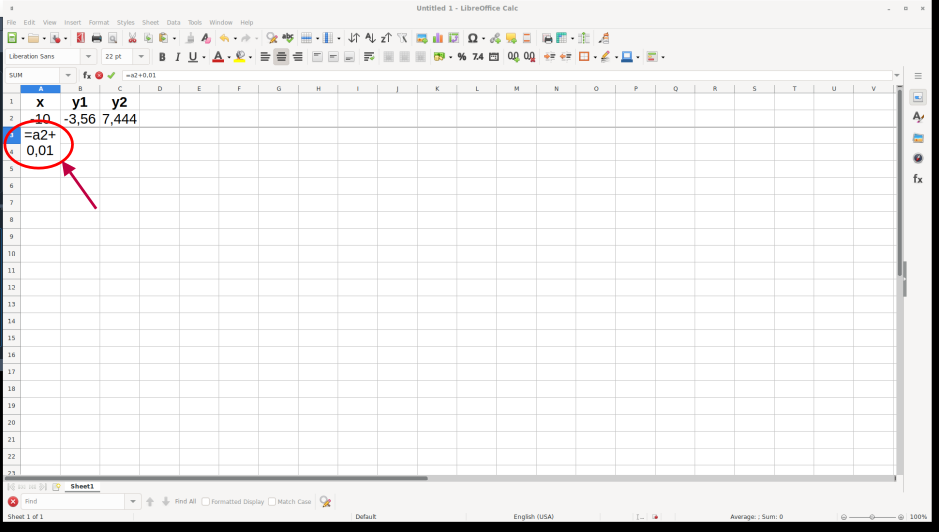
\includegraphics[width=8.0in]{pictures/picture_008.png}
  	\caption{LibreOffice Calc}
   	\label{fig:LibreOfficeCalc008}
\end{figure}
\pict{008}


Poi selezioniamo le caselle $B2$ e $C2$ (figura \ref{fig:LibreOfficeCalc009}). Cliccando sul quadratino in basso a destra e tenendo premuto fino a scorrere alle due caselle di sotto, dovremmo ottenere il risultato della figura \ref{fig:LibreOfficeCalc010}.

Con questo passaggio, le formule matematiche scritte in $B2$ e in $C2$ in funzione della variabile $x$ (figura \ref{fig:LibreOfficeCalc009}) vengono copiate in $B3$ e $C3$ rispettivamente $A3$.

%\begin{figure}[h!]		
	\centering
   	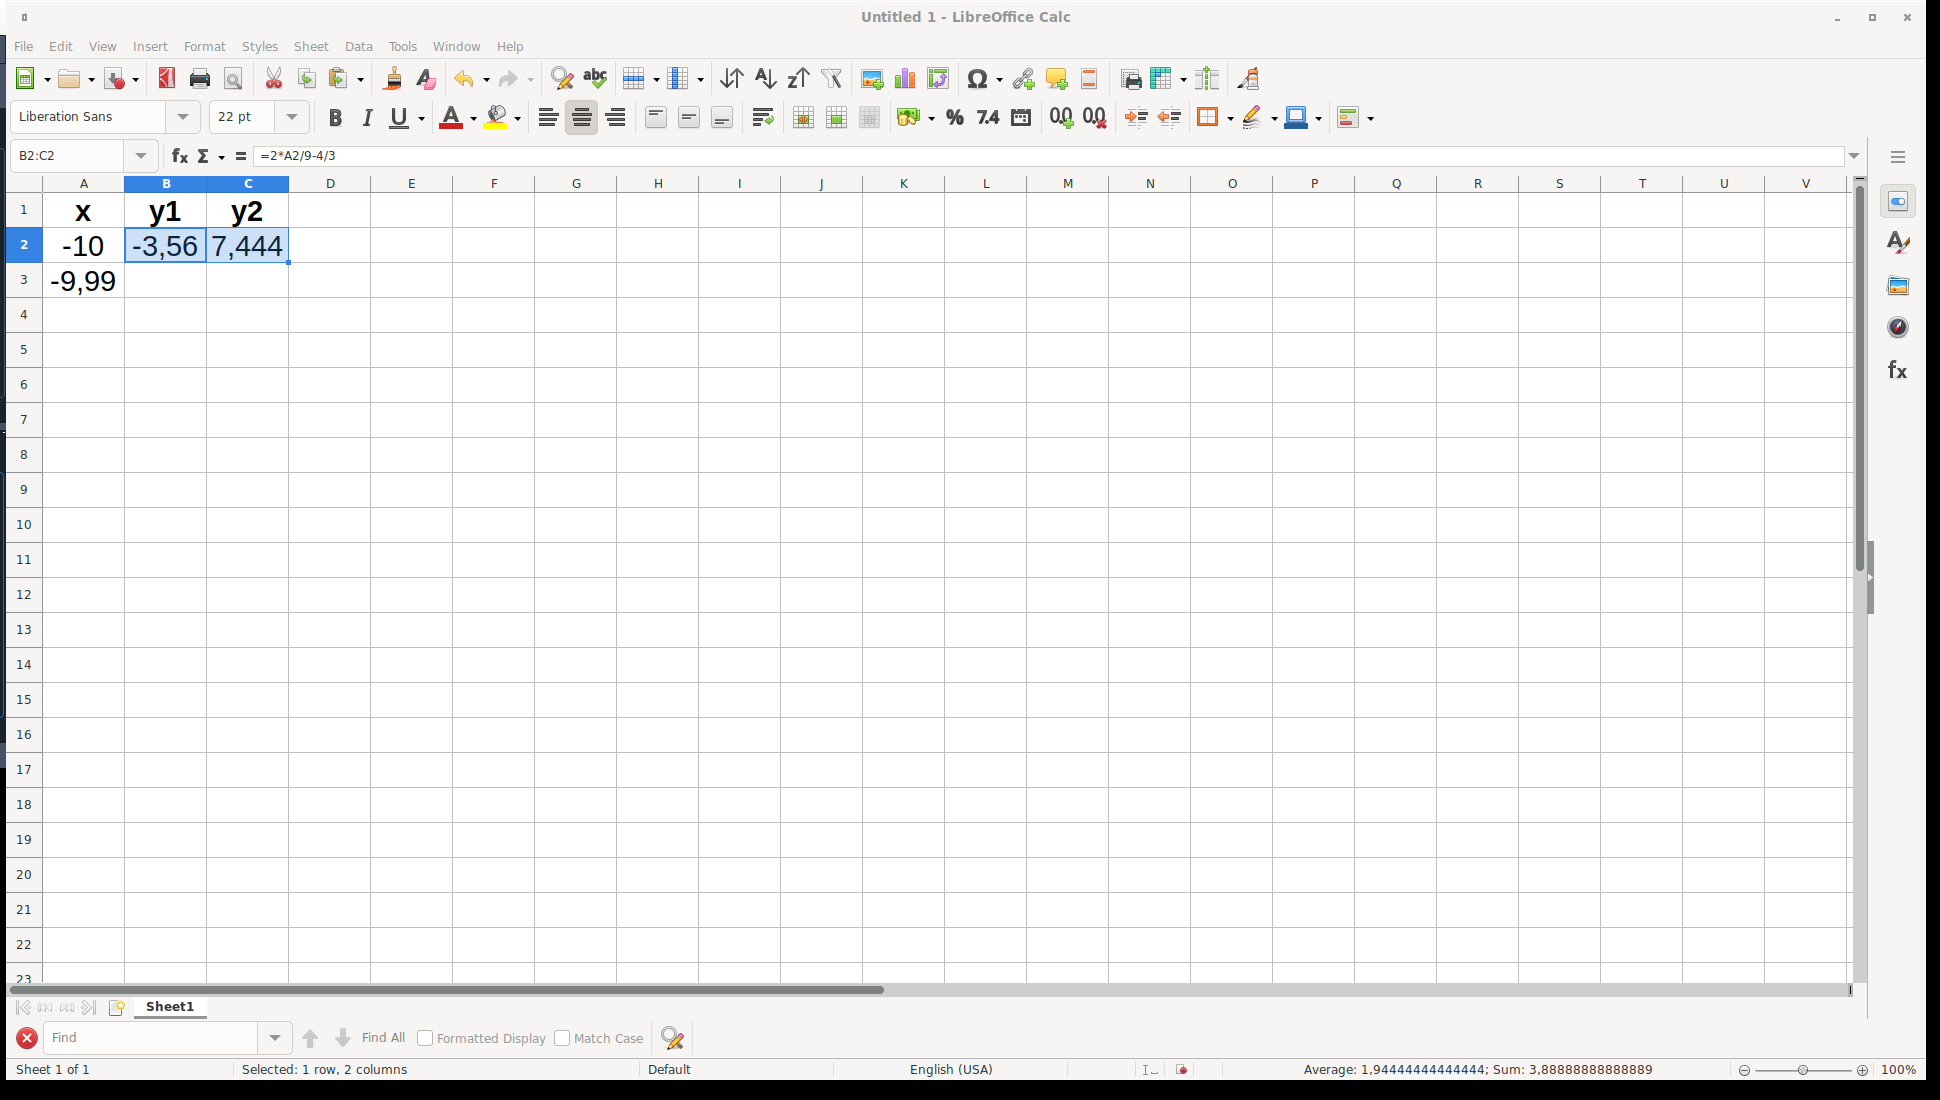
\includegraphics[width=8.0in]{pictures/picture_009.png}
  	\caption{LibreOffice Calc}
   	\label{fig:LibreOfficeCalc009}
\end{figure}
\pict{009}

%\begin{figure}[h!]		
	\centering
   	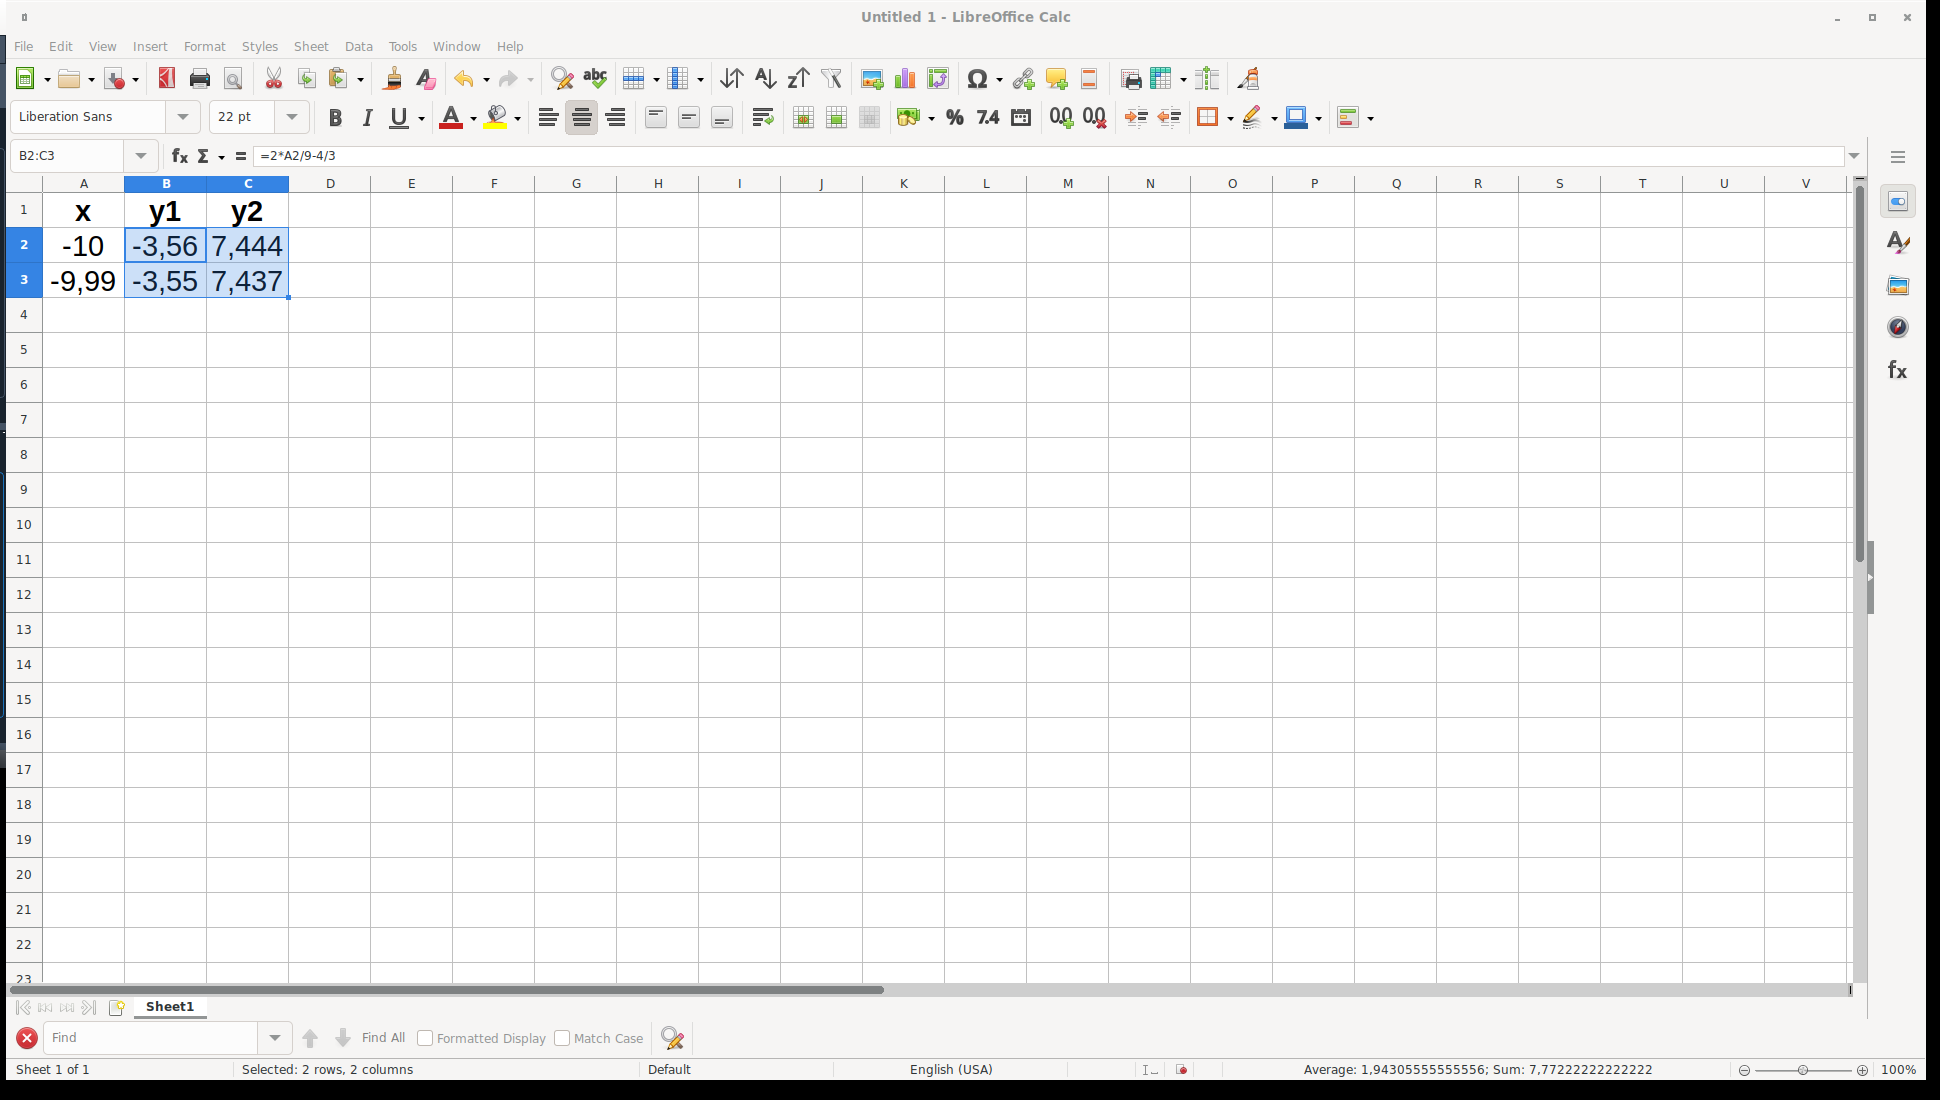
\includegraphics[width=8.0in]{pictures/picture_010.png}
  	\caption{LibreOffice Calc}
   	\label{fig:LibreOfficeCalc010}
\end{figure}
\pict{010}

Selezioniamo ora le caselle $A3$, $B3$ e $C3$, come in figura \ref{fig:LibreOfficeCalc011}

%\begin{figure}[h!]		
	\centering
   	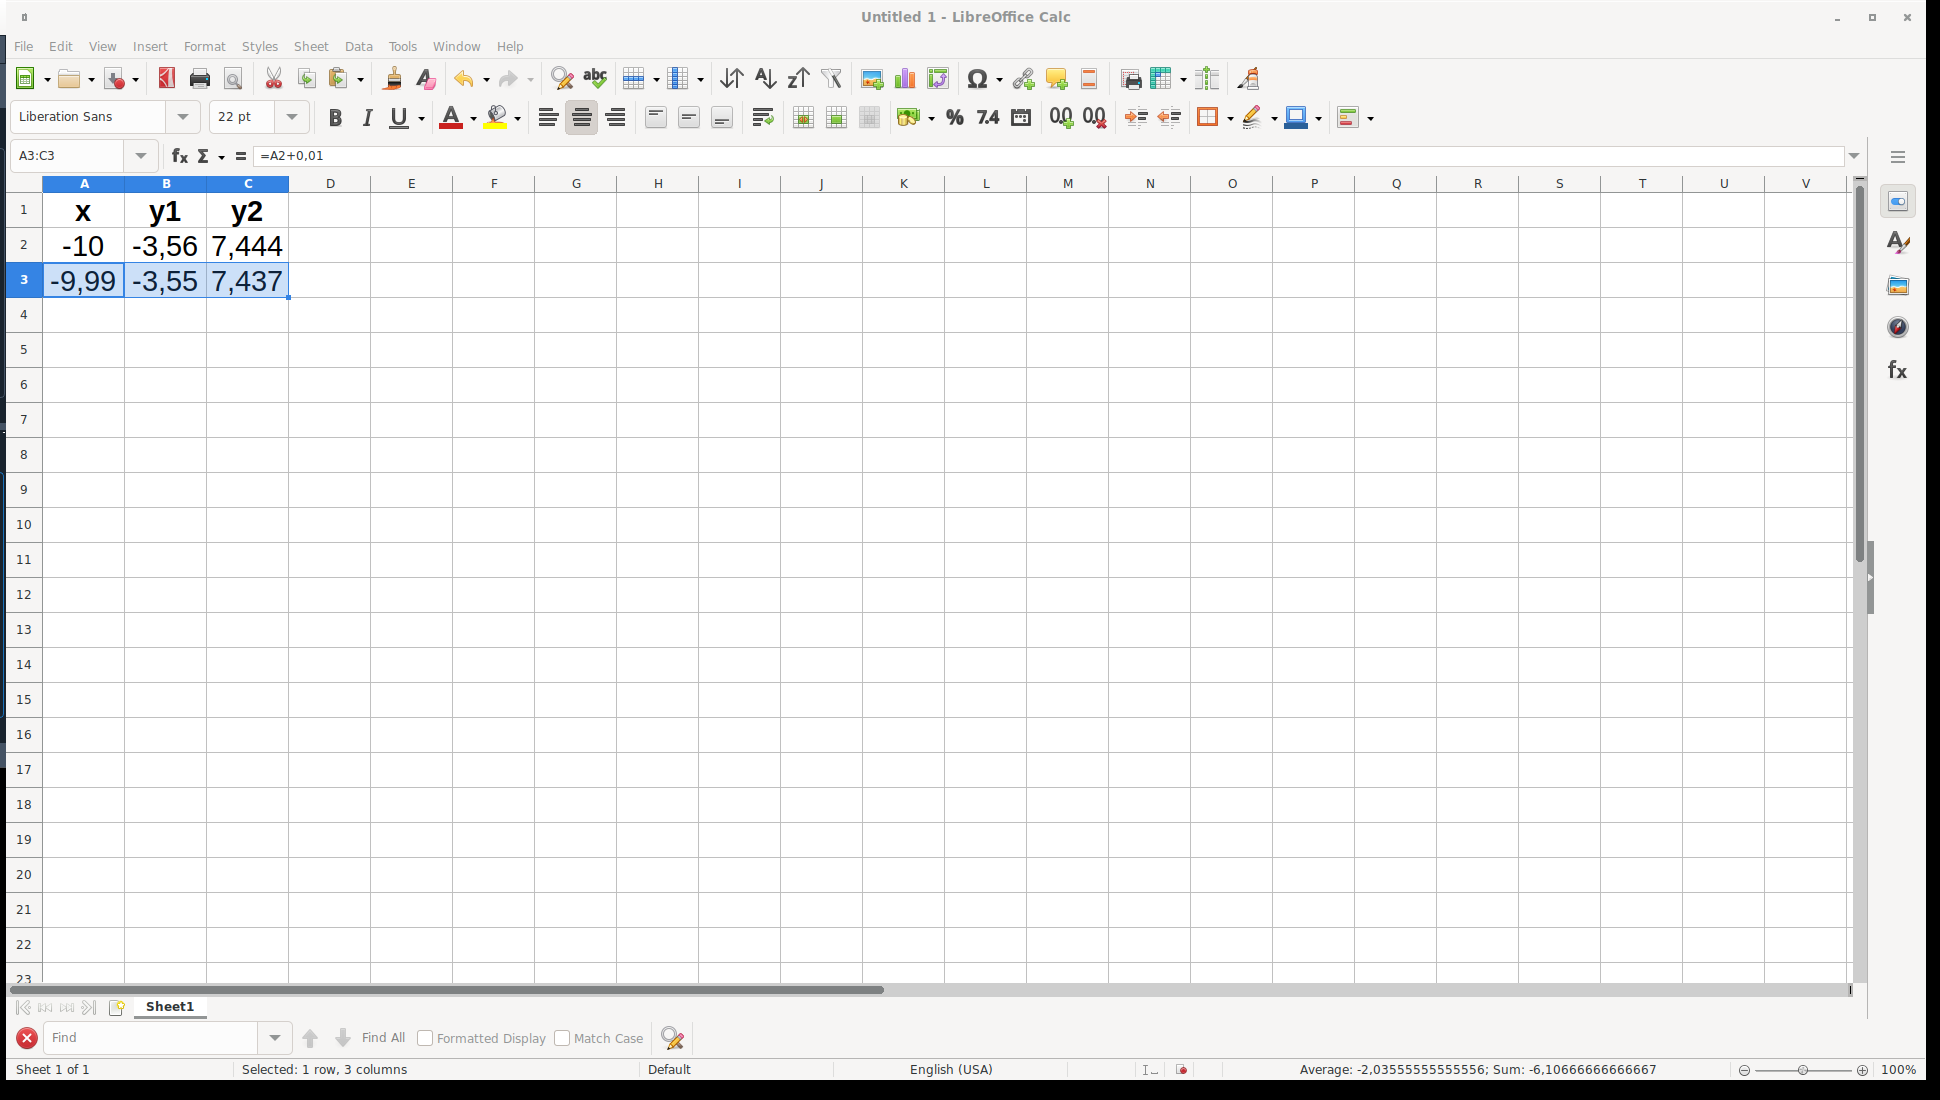
\includegraphics[width=8.0in]{pictures/picture_011.png}
  	\caption{LibreOffice Calc}
   	\label{fig:LibreOfficeCalc011}
\end{figure}
\pict{011}

e ripetiamo il passaggio precedente, copiando le rispettive formule matematiche, non su una riga soltanto, ma per un numero di righe sufficientemente grande da arrivare fino a $x = 10$ (figura \ref{fig:LibreOfficeCalc012}).

%\begin{figure}[h!]		
	\centering
   	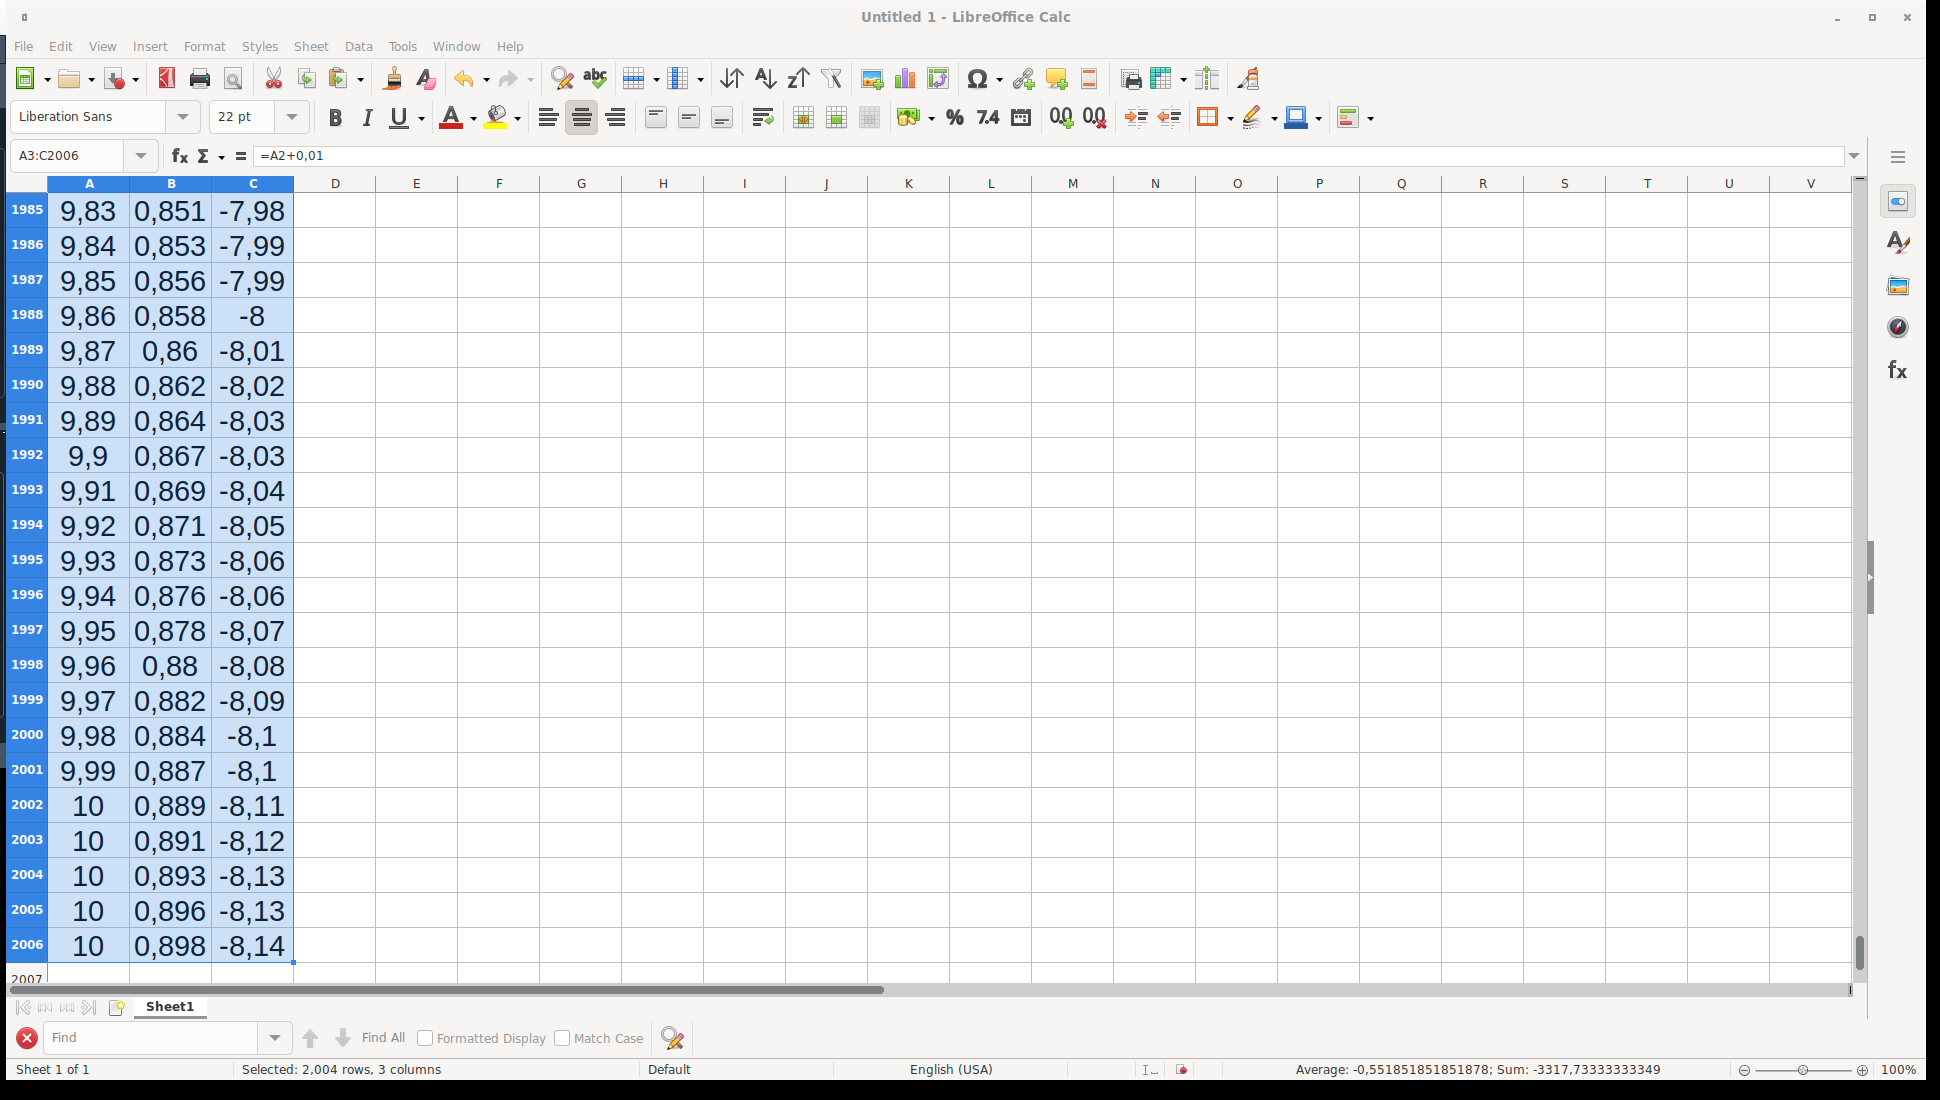
\includegraphics[width=8.0in]{pictures/picture_012.png}
  	\caption{LibreOffice Calc}
   	\label{fig:LibreOfficeCalc012}
\end{figure}
\pict{012}

In questo modo LibreOffice Calc ha eseguito ben 200 calcoli, e con estrema rapidità.


\section{Eseguire il grafico}


Eseguire i seguenti step per riportare le rette associate alle due equazioni del sistema in un unico grafico:

\begin{enumerate}
	\item tornare in alto sul foglio elettronico e selezionare le tre colonne $A$, $B$ e $C$, come in figura 
	
	%\begin{figure}[h!]		
	\centering
   	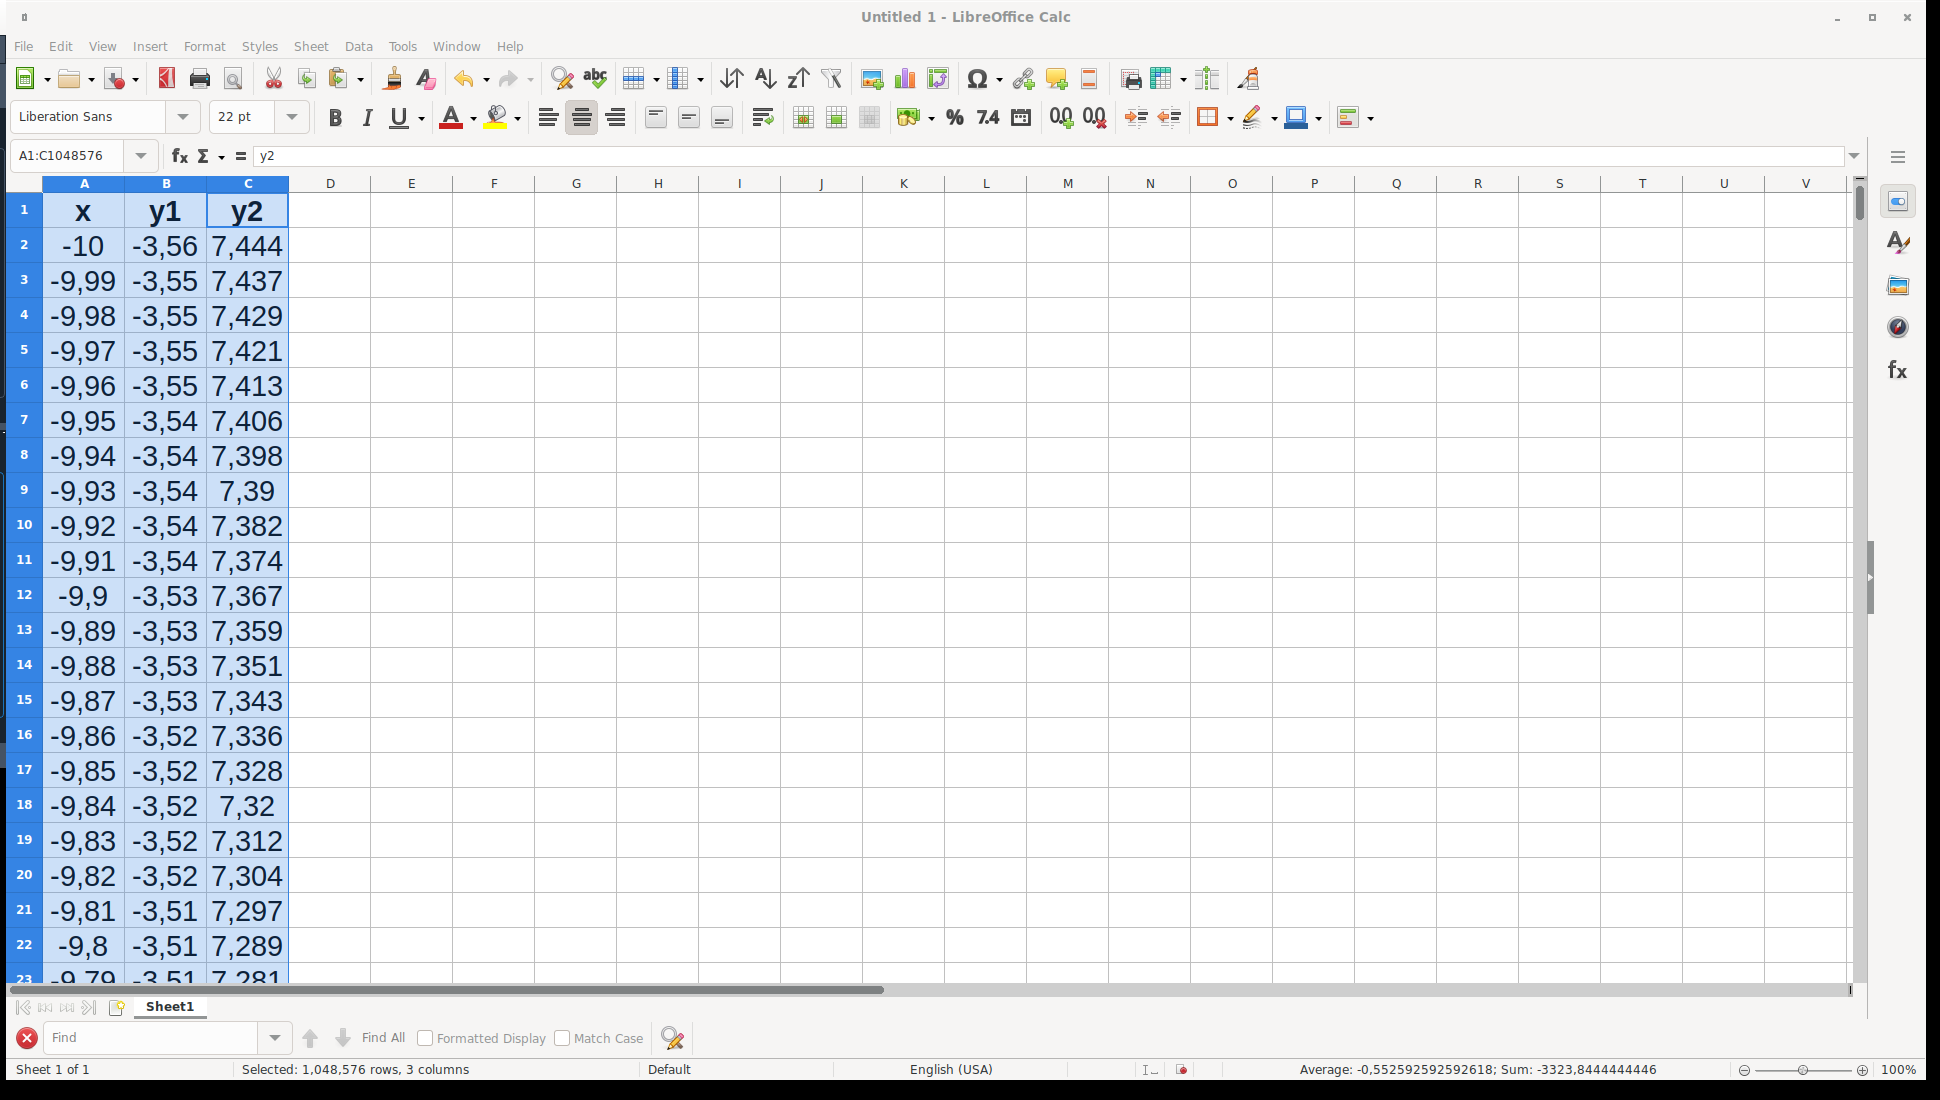
\includegraphics[width=8.0in]{pictures/picture_013.png}
  	\caption{LibreOffice Calc}
   	\label{fig:LibreOfficeCalc013}
\end{figure}
	\pict{013}	
		
	\item Nel menù in alto selezionare "insert -> chart", figura \ref{fig:LibreOfficeCalc014}. Attendere un po' se il computer non è molto prestante.
	
	%\begin{figure}[h!]		
	\centering
   	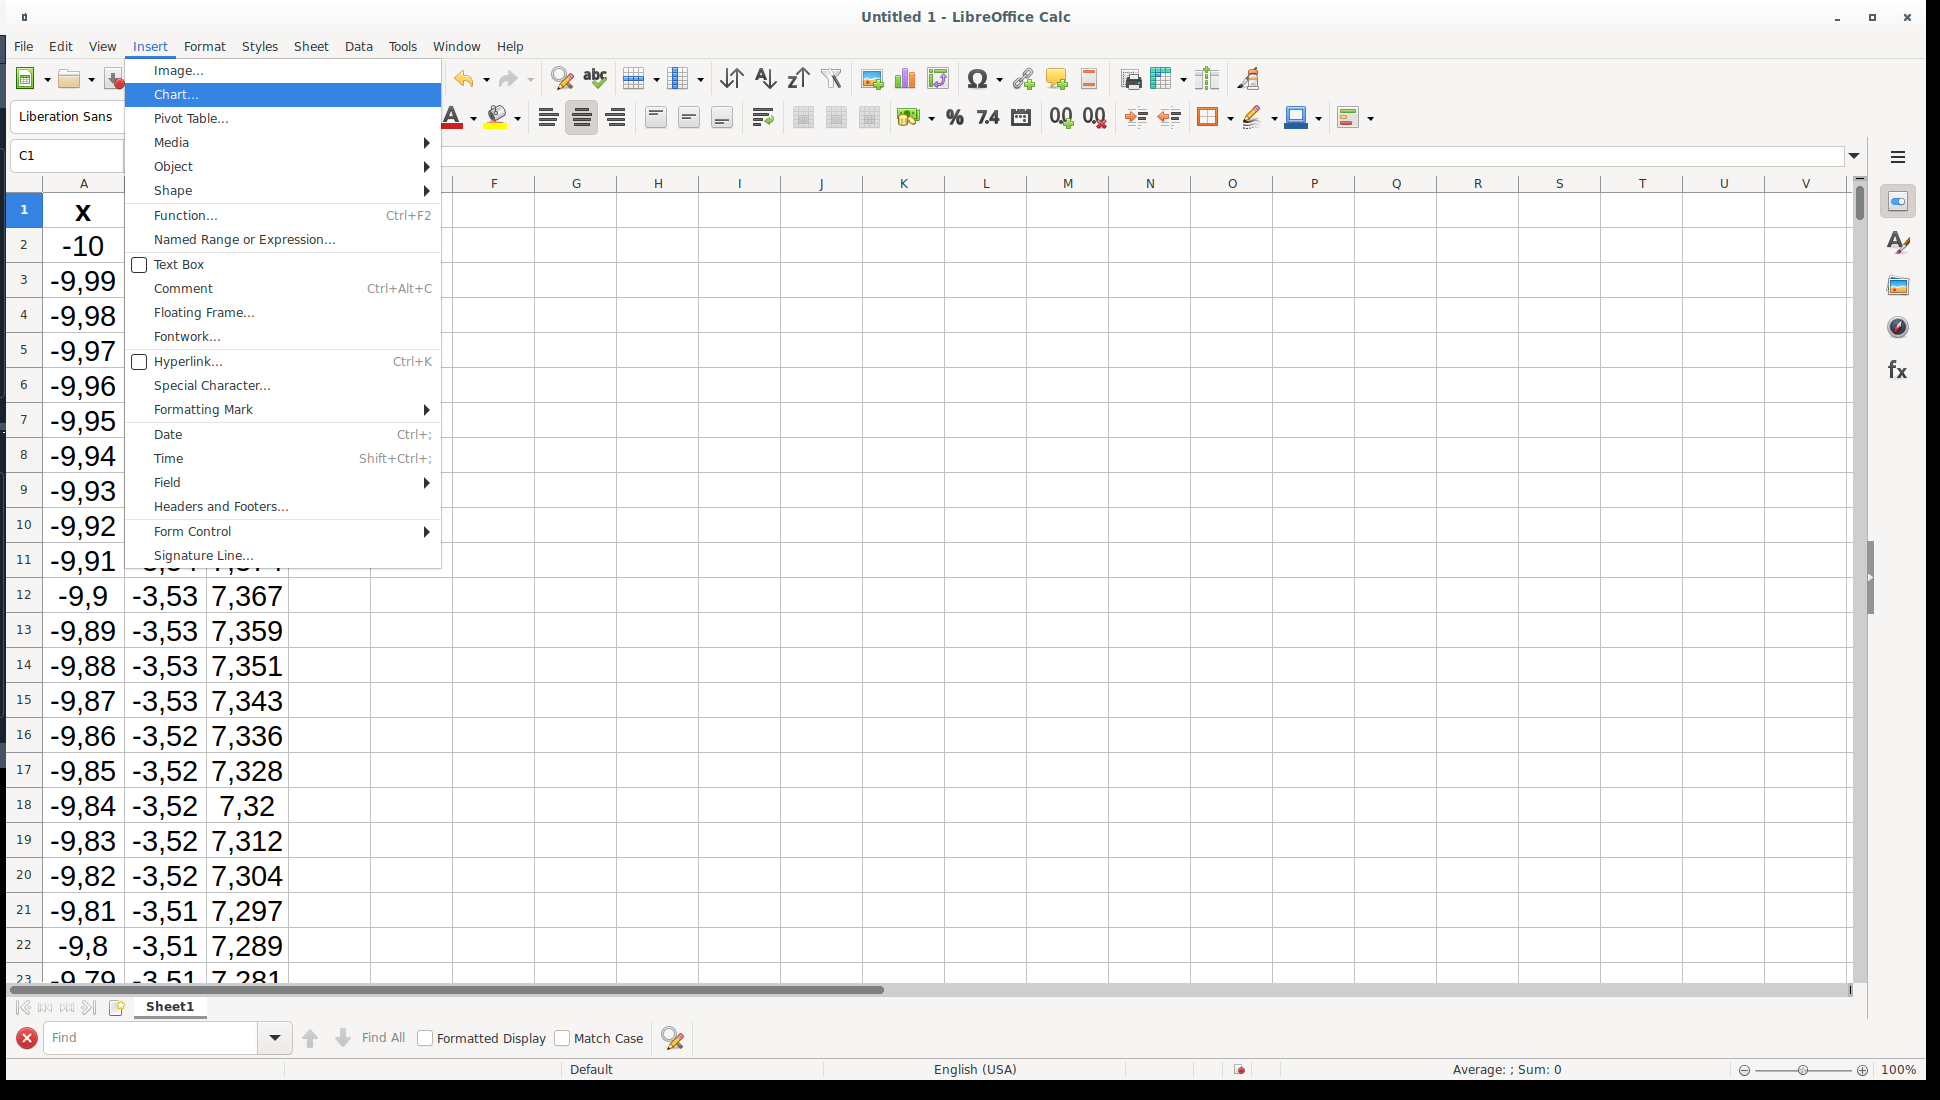
\includegraphics[width=8.0in]{pictures/picture_014.png}
  	\caption{LibreOffice Calc}
   	\label{fig:LibreOfficeCalc014}
\end{figure}
	\pict{014}	
	
	\item Selezionare "XY (Scatter)" nella finestra che si apre e, successivamente, "Lines Only" nel riquadro a fianco, e infine premere su "finish".
	
	%\begin{figure}[h!]		
	\centering
   	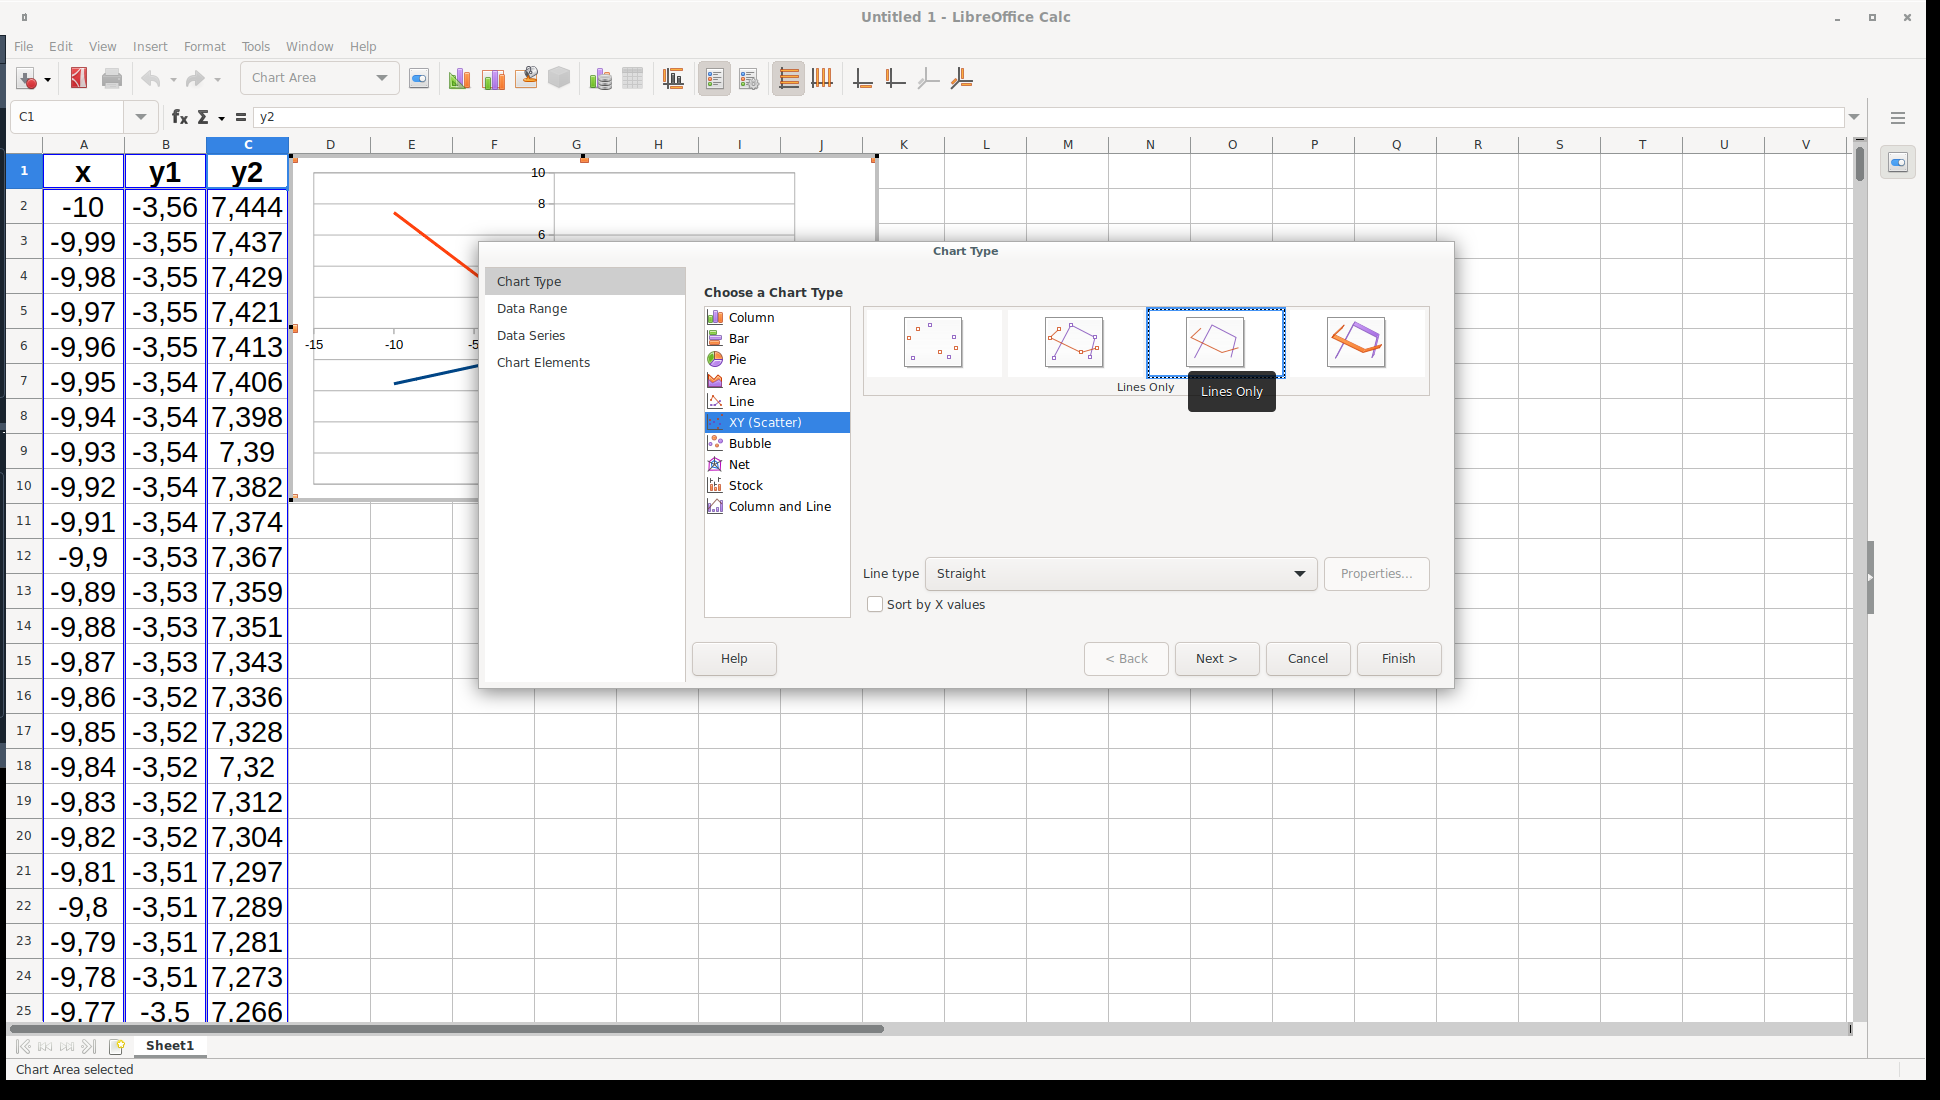
\includegraphics[width=8.0in]{pictures/picture_015.png}
  	\caption{LibreOffice Calc}
   	\label{fig:LibreOfficeCalc015}
\end{figure}
	\pict{015}
	
	\item Il grafico della figura \ref{fig:LibreOfficeCalc016} dovrebbe apparire

	%\begin{figure}[h!]		
	\centering
   	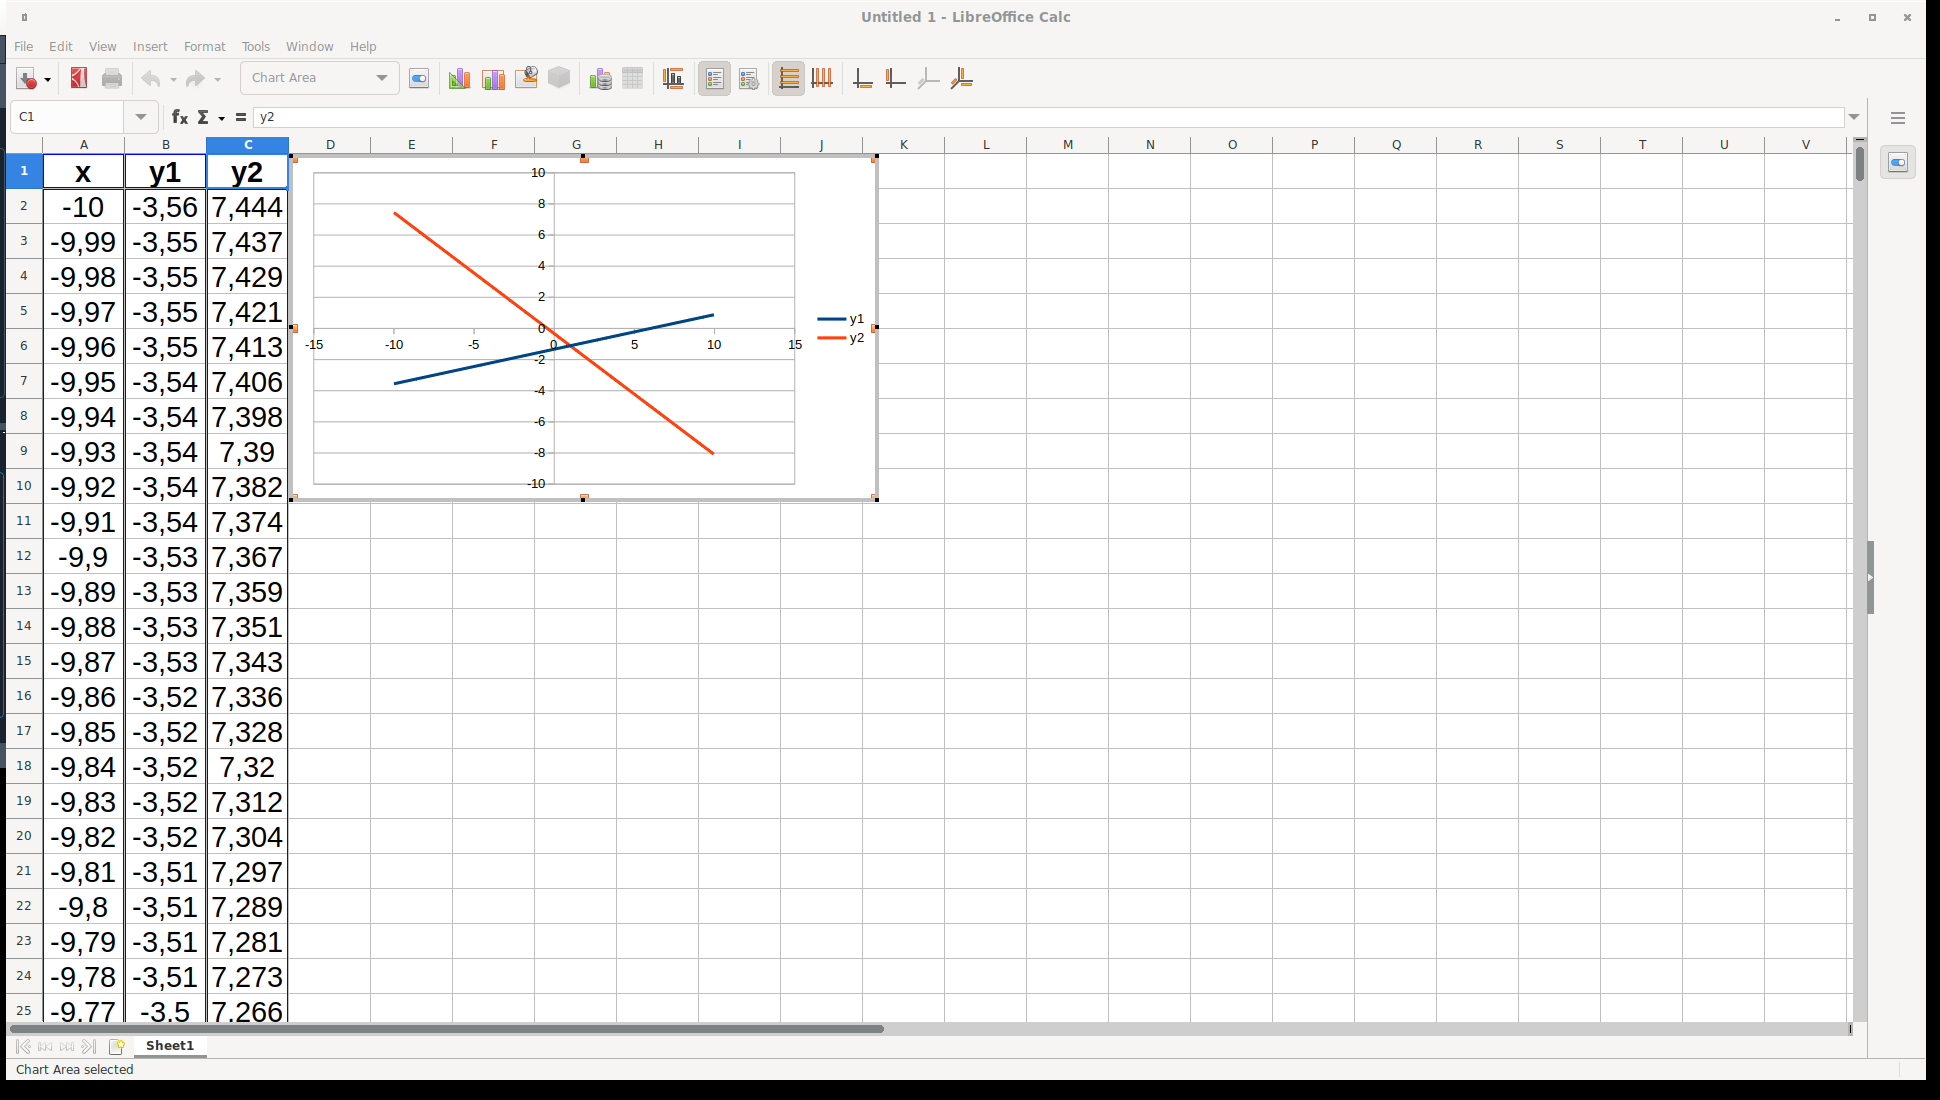
\includegraphics[width=8.0in]{pictures/picture_016.png}
  	\caption{LibreOffice Calc}
   	\label{fig:LibreOfficeCalc016}
\end{figure}
	\pict{016}

\end{enumerate}
Il punto di intersezione delle due rette dovrebbe avere, appunto, come coordinate la risoluzione del sistema eq. \ref{eq:sistema} o, parimenti, del sistema \ref{eq:sistemaEspl}. Il problema, però, è che questo grafico \emph{non} ha una griglia abbastanza fitta e l'analisi, fino a questo punto, può essere fatta solo in linea di massima. Possiamo allargare il grafico andando a cliccare sui quadratini agli angoli del riquadro che lo delimita (figura \ref{fig:LibreOfficeCalc017}


%\begin{figure}[h!]		
	\centering
   	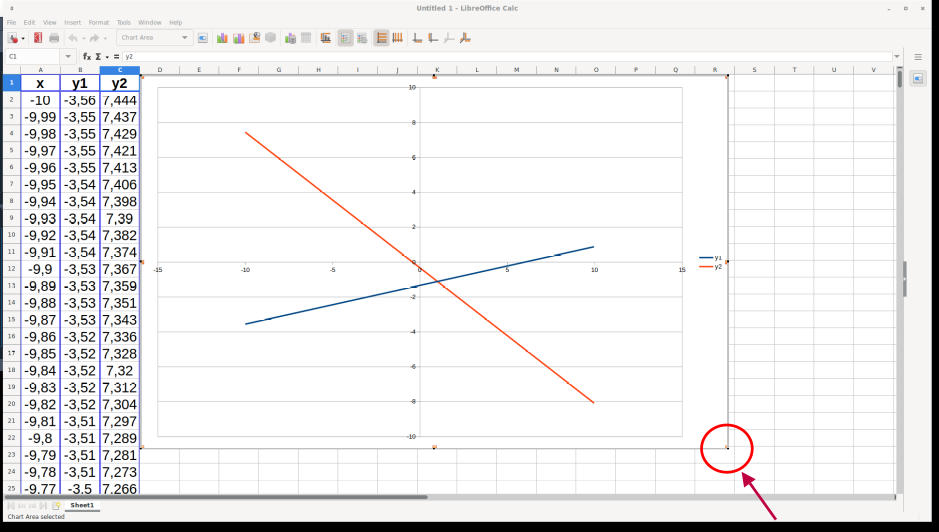
\includegraphics[width=8.0in]{pictures/picture_017.png}
  	\caption{LibreOffice Calc}
   	\label{fig:LibreOfficeCalc017}
\end{figure}
\pict{017}


Andiamo a vedere come si possono impostare i parametri del grafico, in modo da accertarci che il punto di intersezione sia effettivamente quello cercato.




\section{Impostazione dei parametri del grafico}

In primo luogo notiamo che i valori delle $x$ vanno da $-15$ a $+15$, mentre a noi basta che vadano da $-10$ a $+10$. Nella figura \ref{fig:LibreOfficeCalc017} facciamo doppio click su uno dei numeri dell'asse delle $x$, ad esempio il numero $-5$ e si apre la finestra di figura \ref{fig:LibreOfficeCalc018}

%\begin{figure}[h!]		
	\centering
   	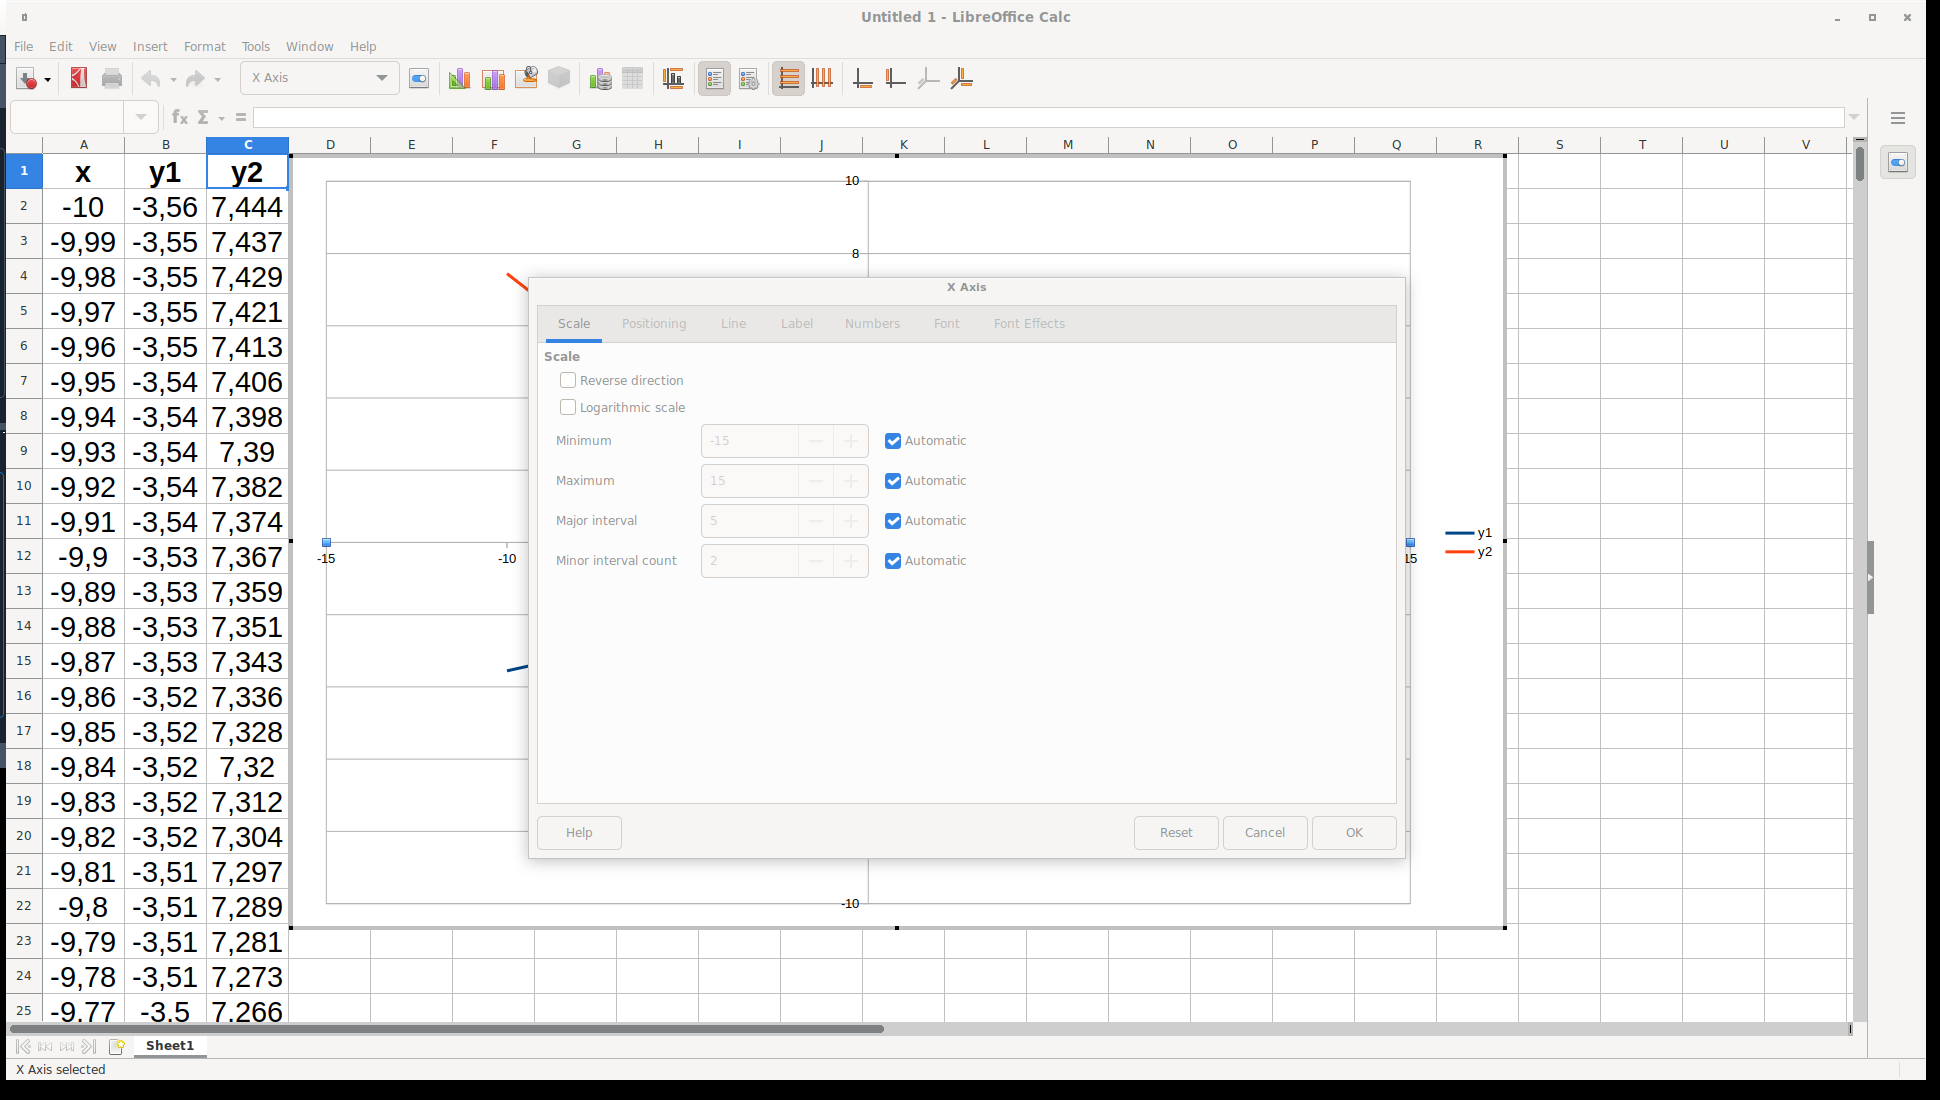
\includegraphics[width=8.0in]{pictures/picture_018.png}
  	\caption{LibreOffice Calc}
   	\label{fig:LibreOfficeCalc018}
\end{figure}
\pict{018}

Leviamo la spunta su "automatic" su tutte e quattro le voci, cambiamo "Minimum" e "Maximum" in $-10$ e $+10$, cambiamo anche "Major interval" e "Minor interval count" in modo da impostare una griglia più vicina a quella di una carta millimetrata, come in figura \ref{fig:LibreOfficeCalc019}


%\begin{figure}[h!]		
	\centering
   	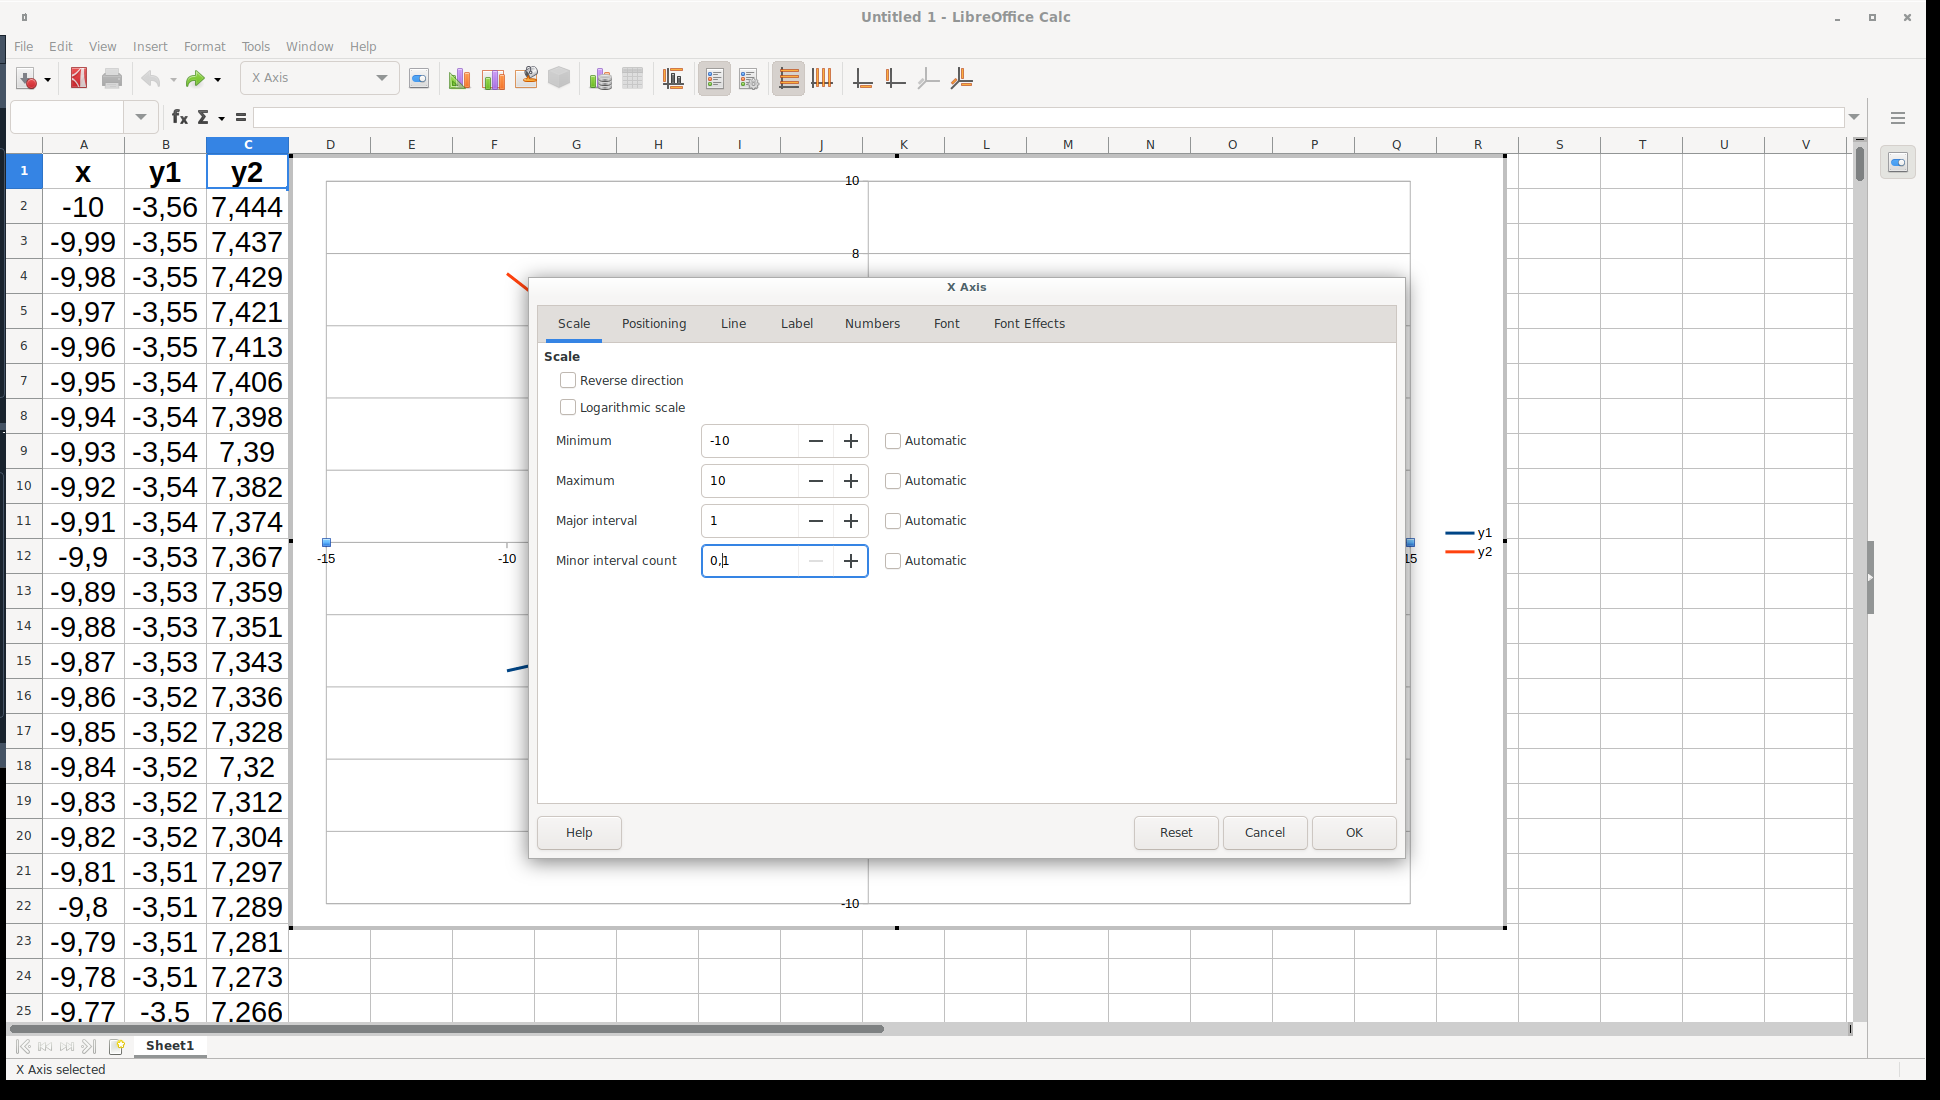
\includegraphics[width=8.0in]{pictures/picture_019.png}
  	\caption{LibreOffice Calc}
   	\label{fig:LibreOfficeCalc019}
\end{figure}
\pict{019}

E il risultato dovrebbe essere quello di figura \ref{fig:LibreOfficeCalc020}

%\begin{figure}[h!]		
	\centering
   	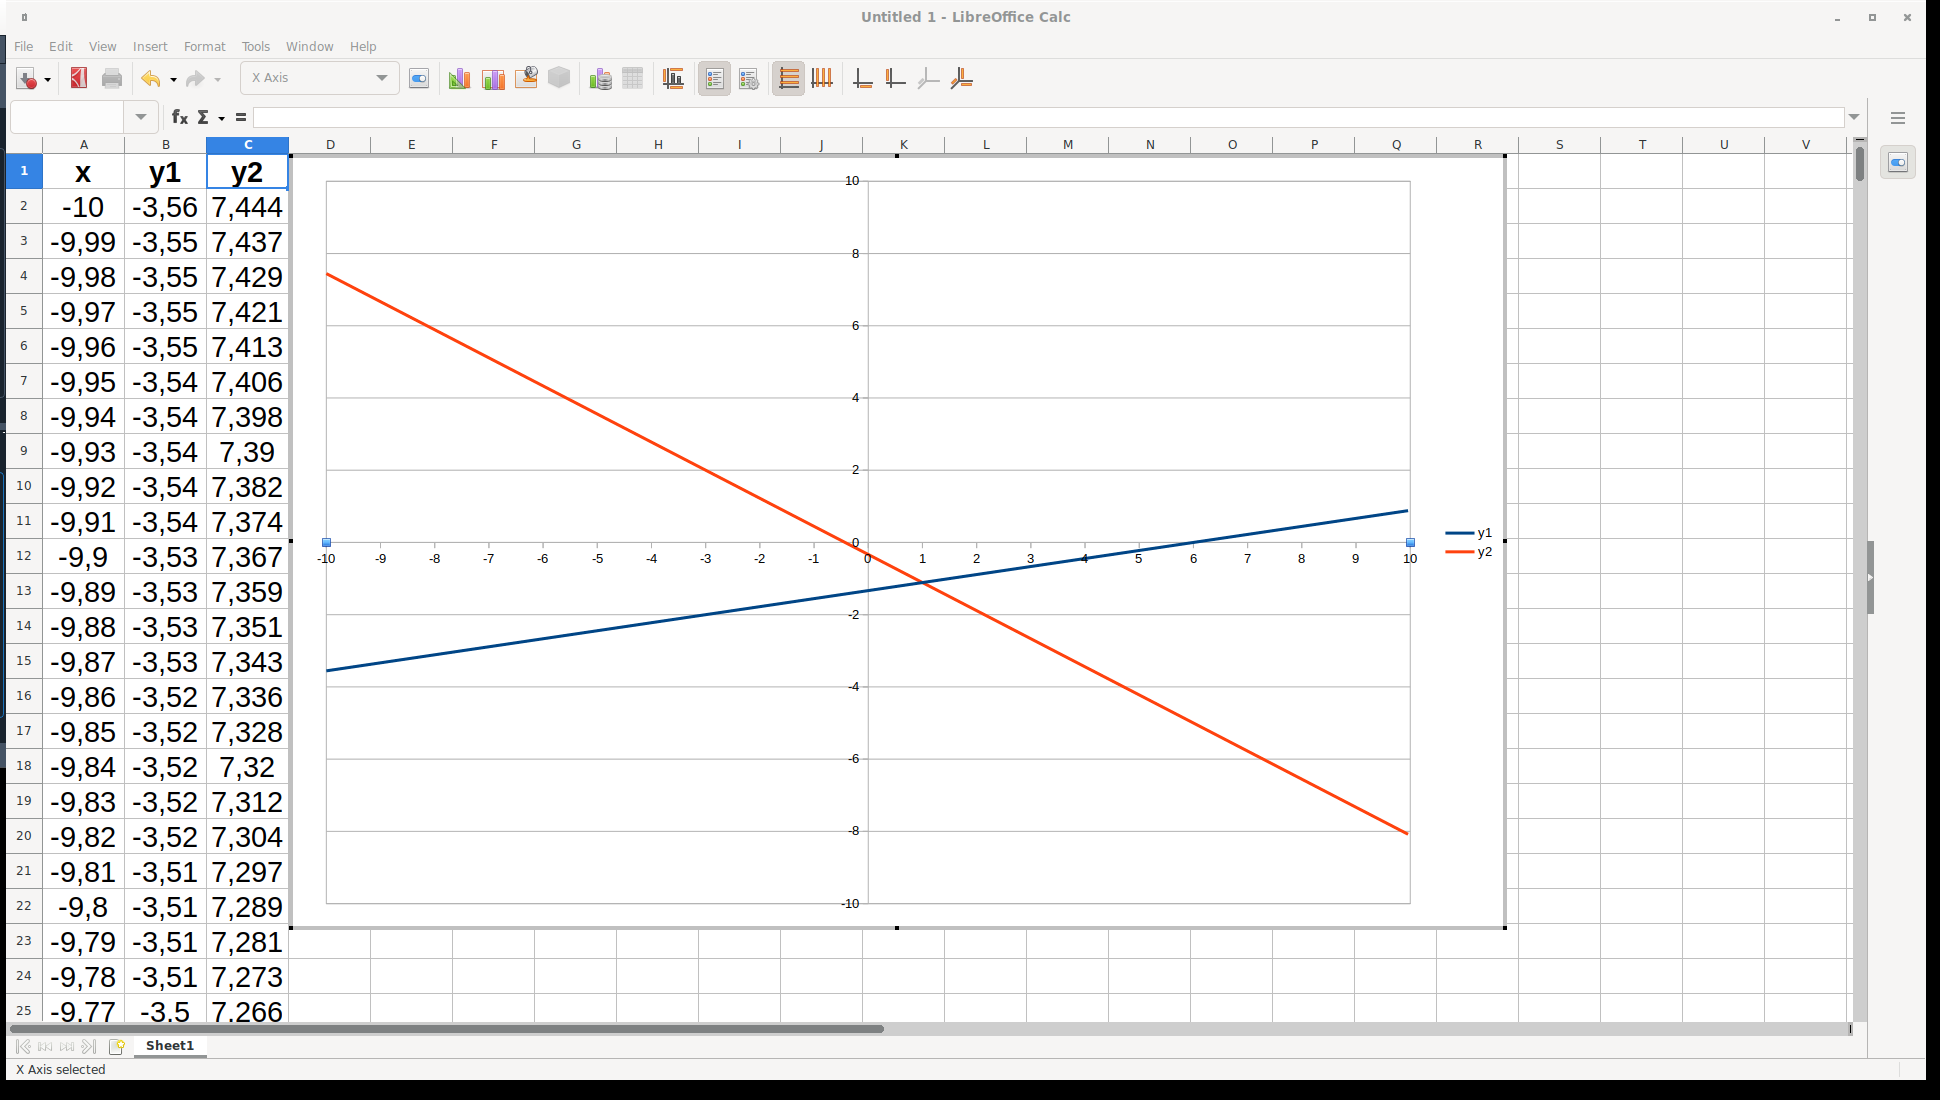
\includegraphics[width=8.0in]{pictures/picture_020.png}
  	\caption{LibreOffice Calc}
   	\label{fig:LibreOfficeCalc020}
\end{figure}
\pict{020}

Allo stesso modo, cliccando su un numero dell'asse delle $y$, ad esempio il numero $2$, si possono configurare i valori massimo e minimo di $y$, nonchè i valori della griglia

\ref{fig:LibreOfficeCalc021}


%\begin{figure}[h!]		
	\centering
   	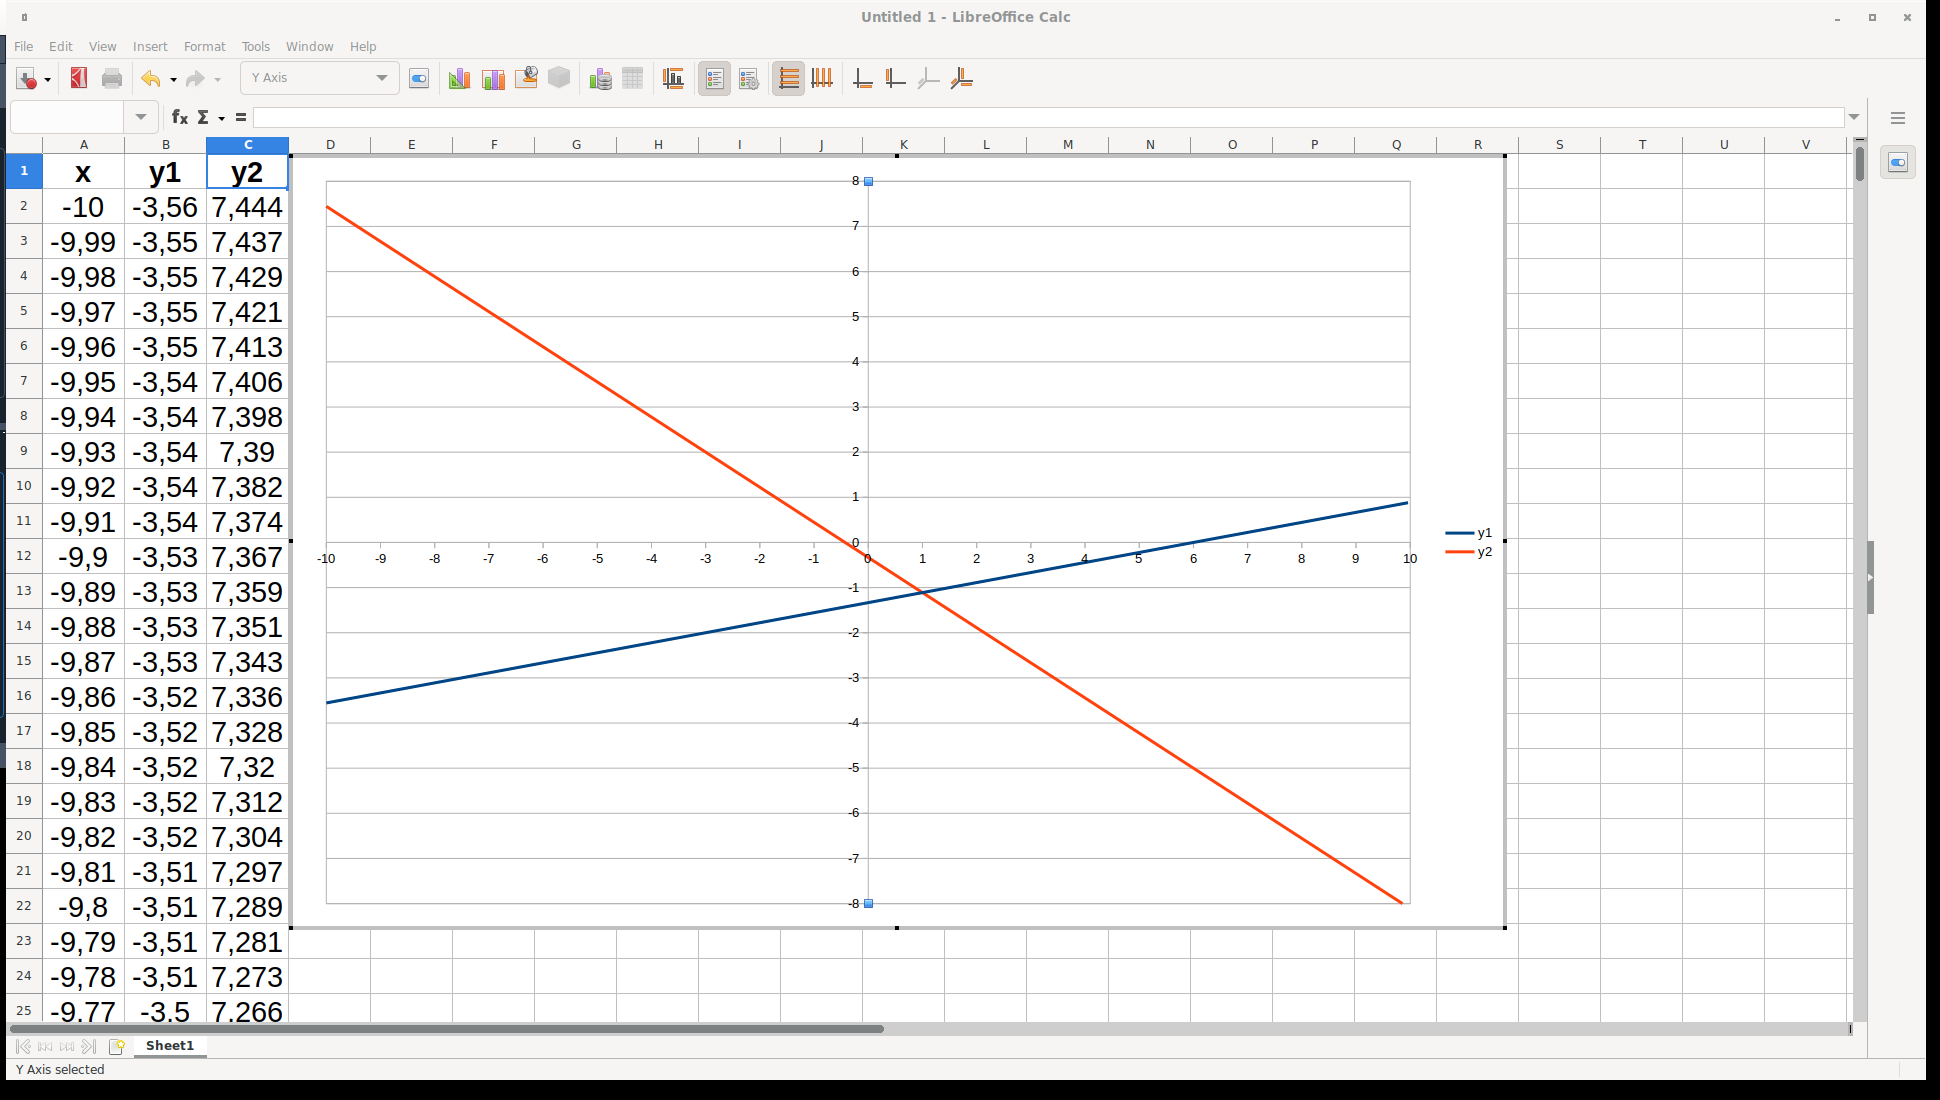
\includegraphics[width=8.0in]{pictures/picture_021.png}
  	\caption{LibreOffice Calc}
   	\label{fig:LibreOfficeCalc021}
\end{figure}
\pict{021}





\section{Cambiare il font dei numeri sugli assi}

Nella figura \ref{fig:LibreOfficeCalc022} risulta che bisogna cliccare prima su font e poi scegliere il valore desiderato.
%\begin{figure}[h!]		
	\centering
   	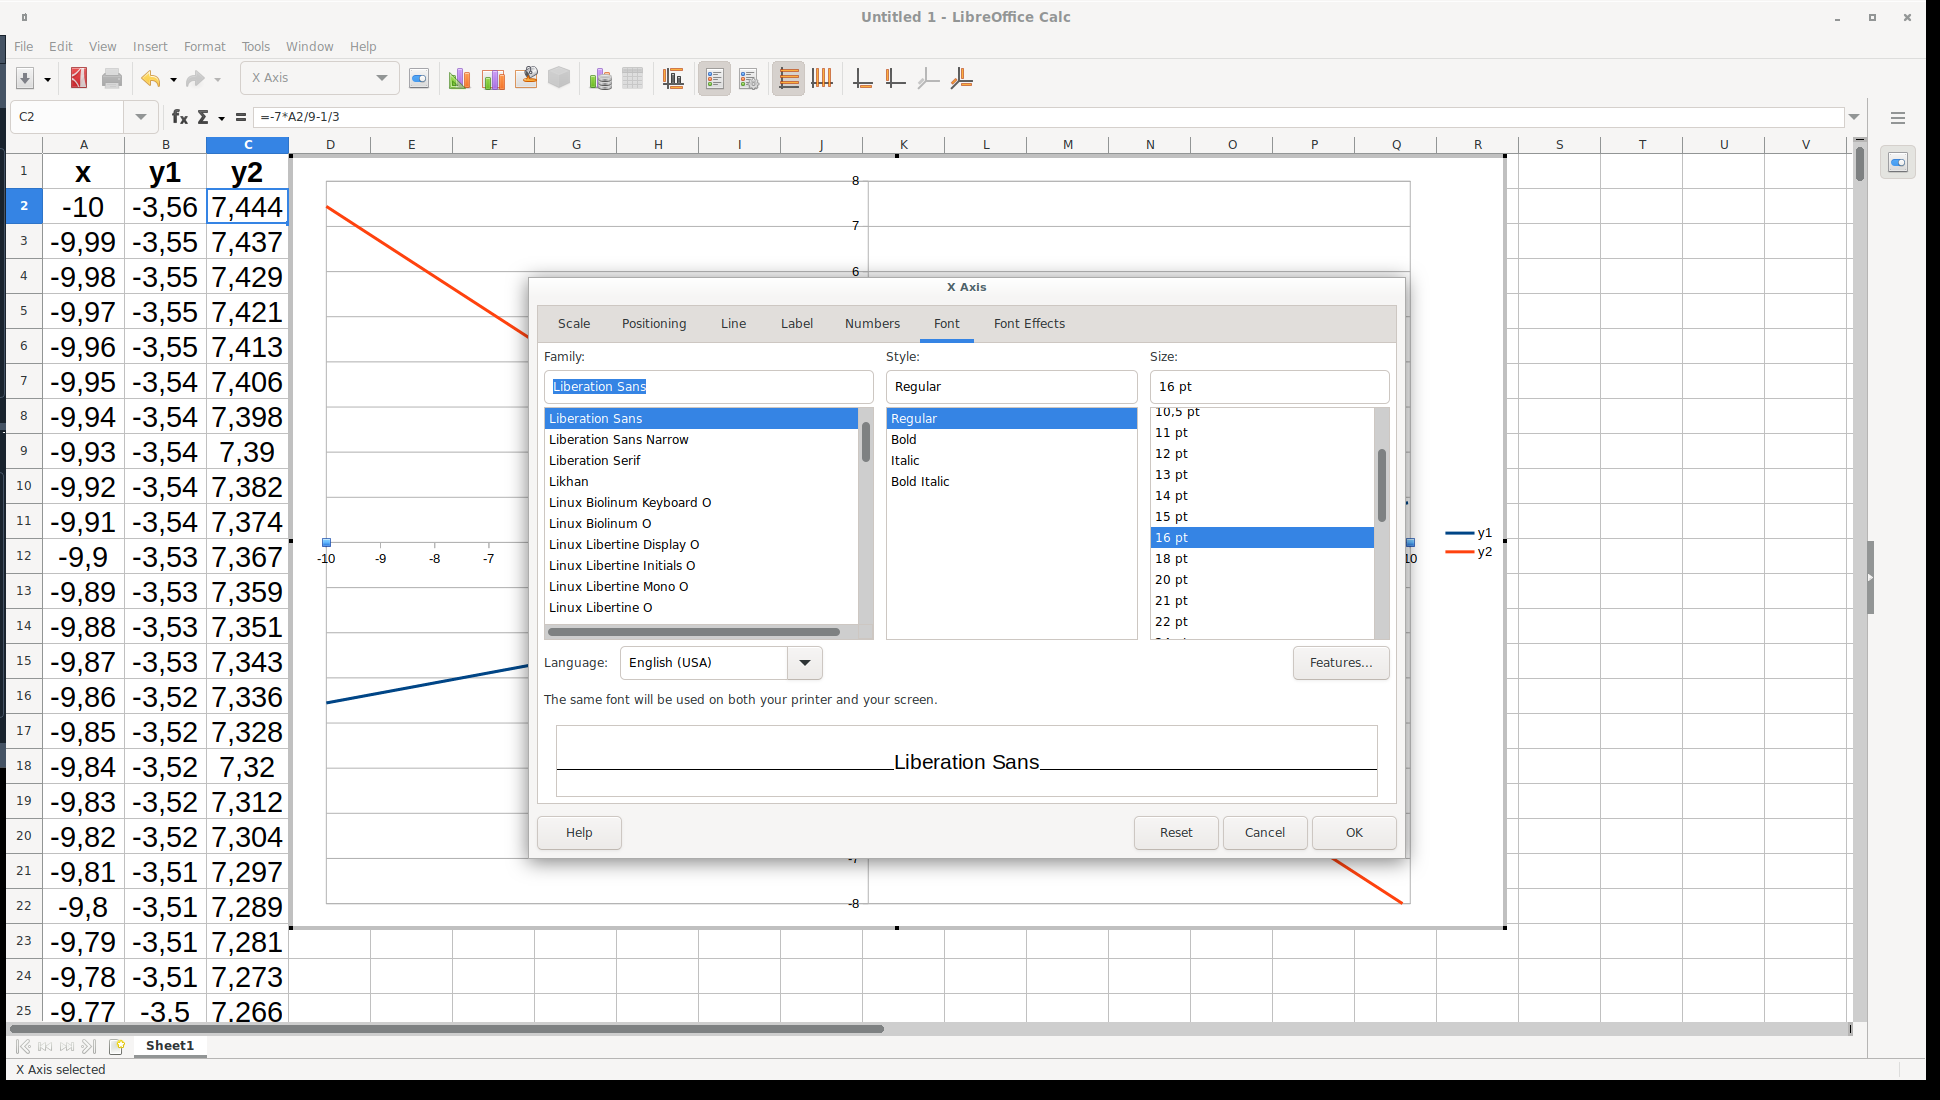
\includegraphics[width=8.0in]{pictures/picture_022.png}
  	\caption{LibreOffice Calc}
   	\label{fig:LibreOfficeCalc022}
\end{figure}
\pict{022}


nella figura \ref{fig:LibreOfficeCalc023} il risultato, dopo aver impostato un font pari a 16 \emph{sia} per i numeri dell'asse delle $x$, sia per i numeri dell'asse delle $y$

%\begin{figure}[h!]		
	\centering
   	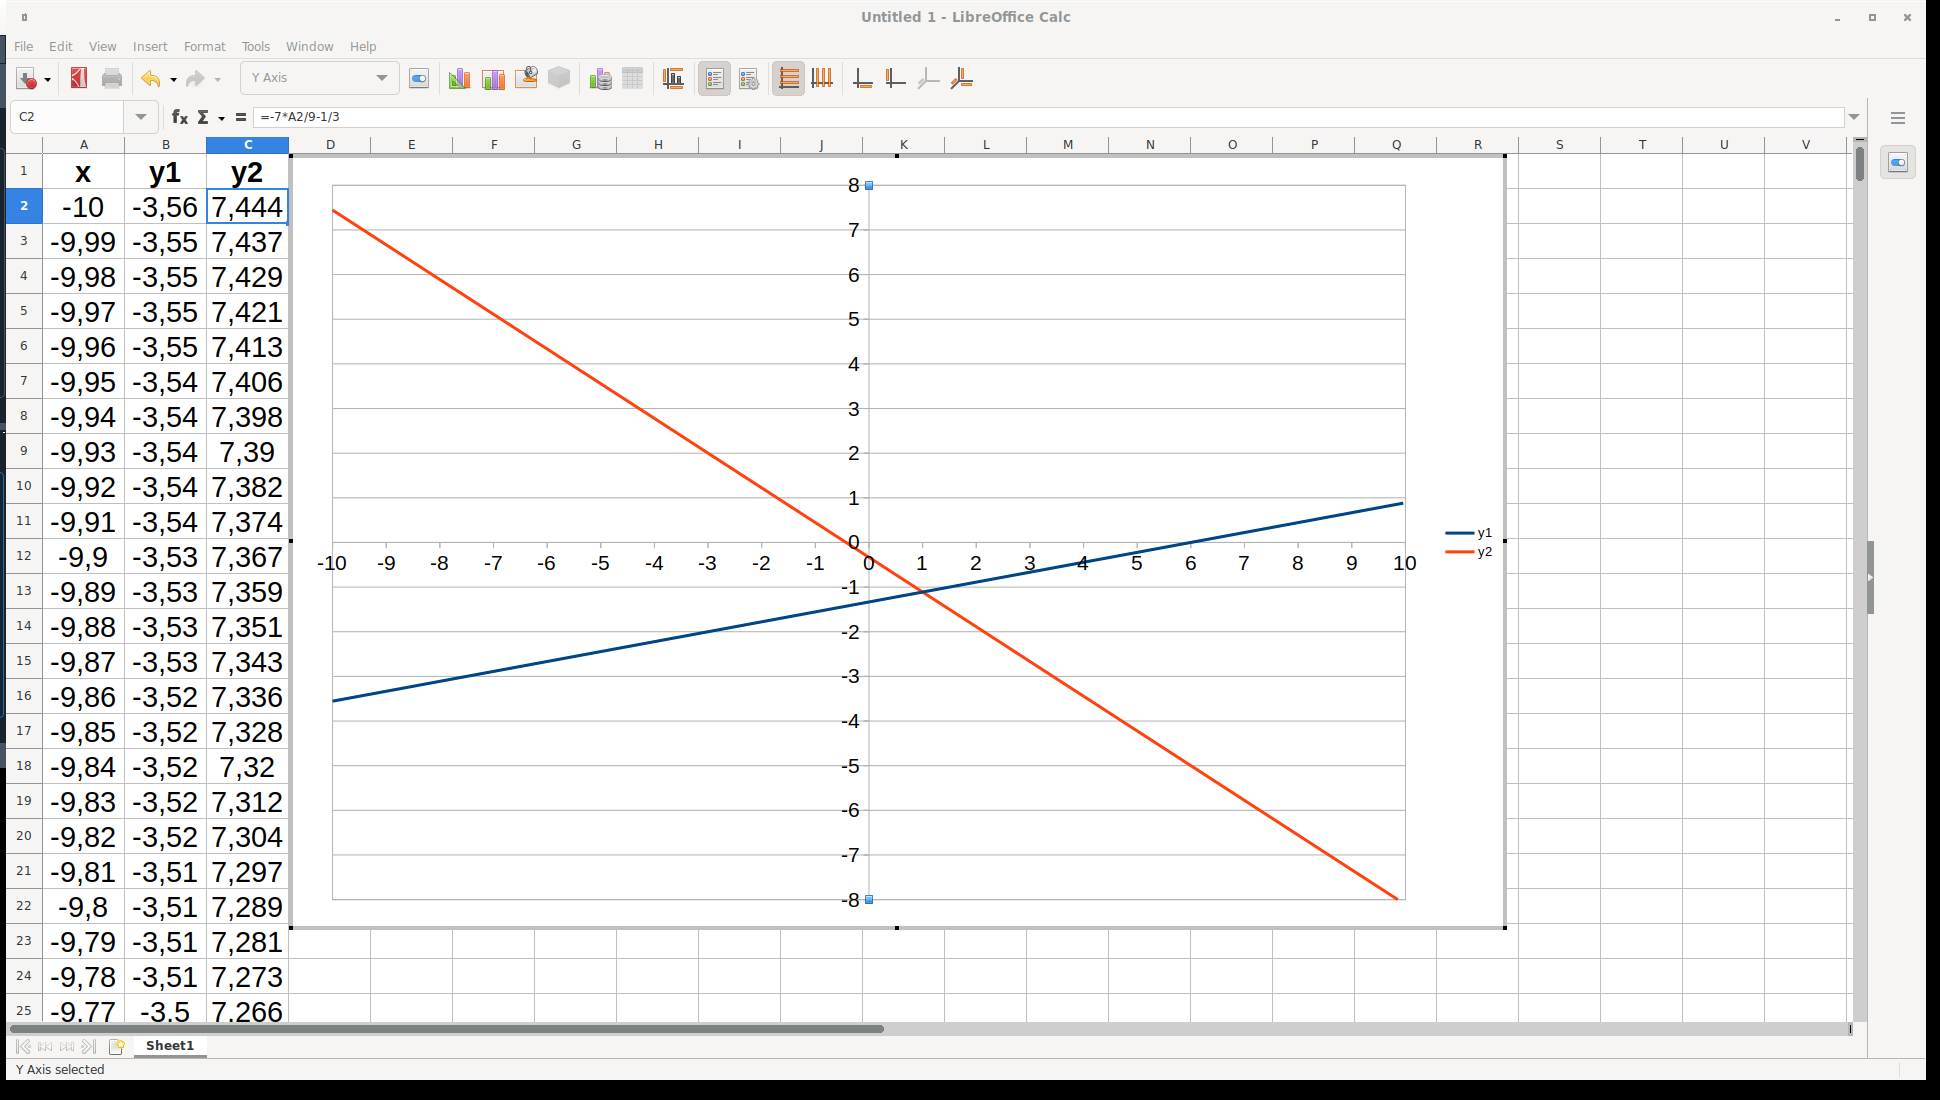
\includegraphics[width=8.0in]{pictures/picture_023.png}
  	\caption{LibreOffice Calc}
   	\label{fig:LibreOfficeCalc023}
\end{figure}
\pict{023}



\section{Inserire una griglia più fitta}

%\begin{figure}[h!]		
	\centering
   	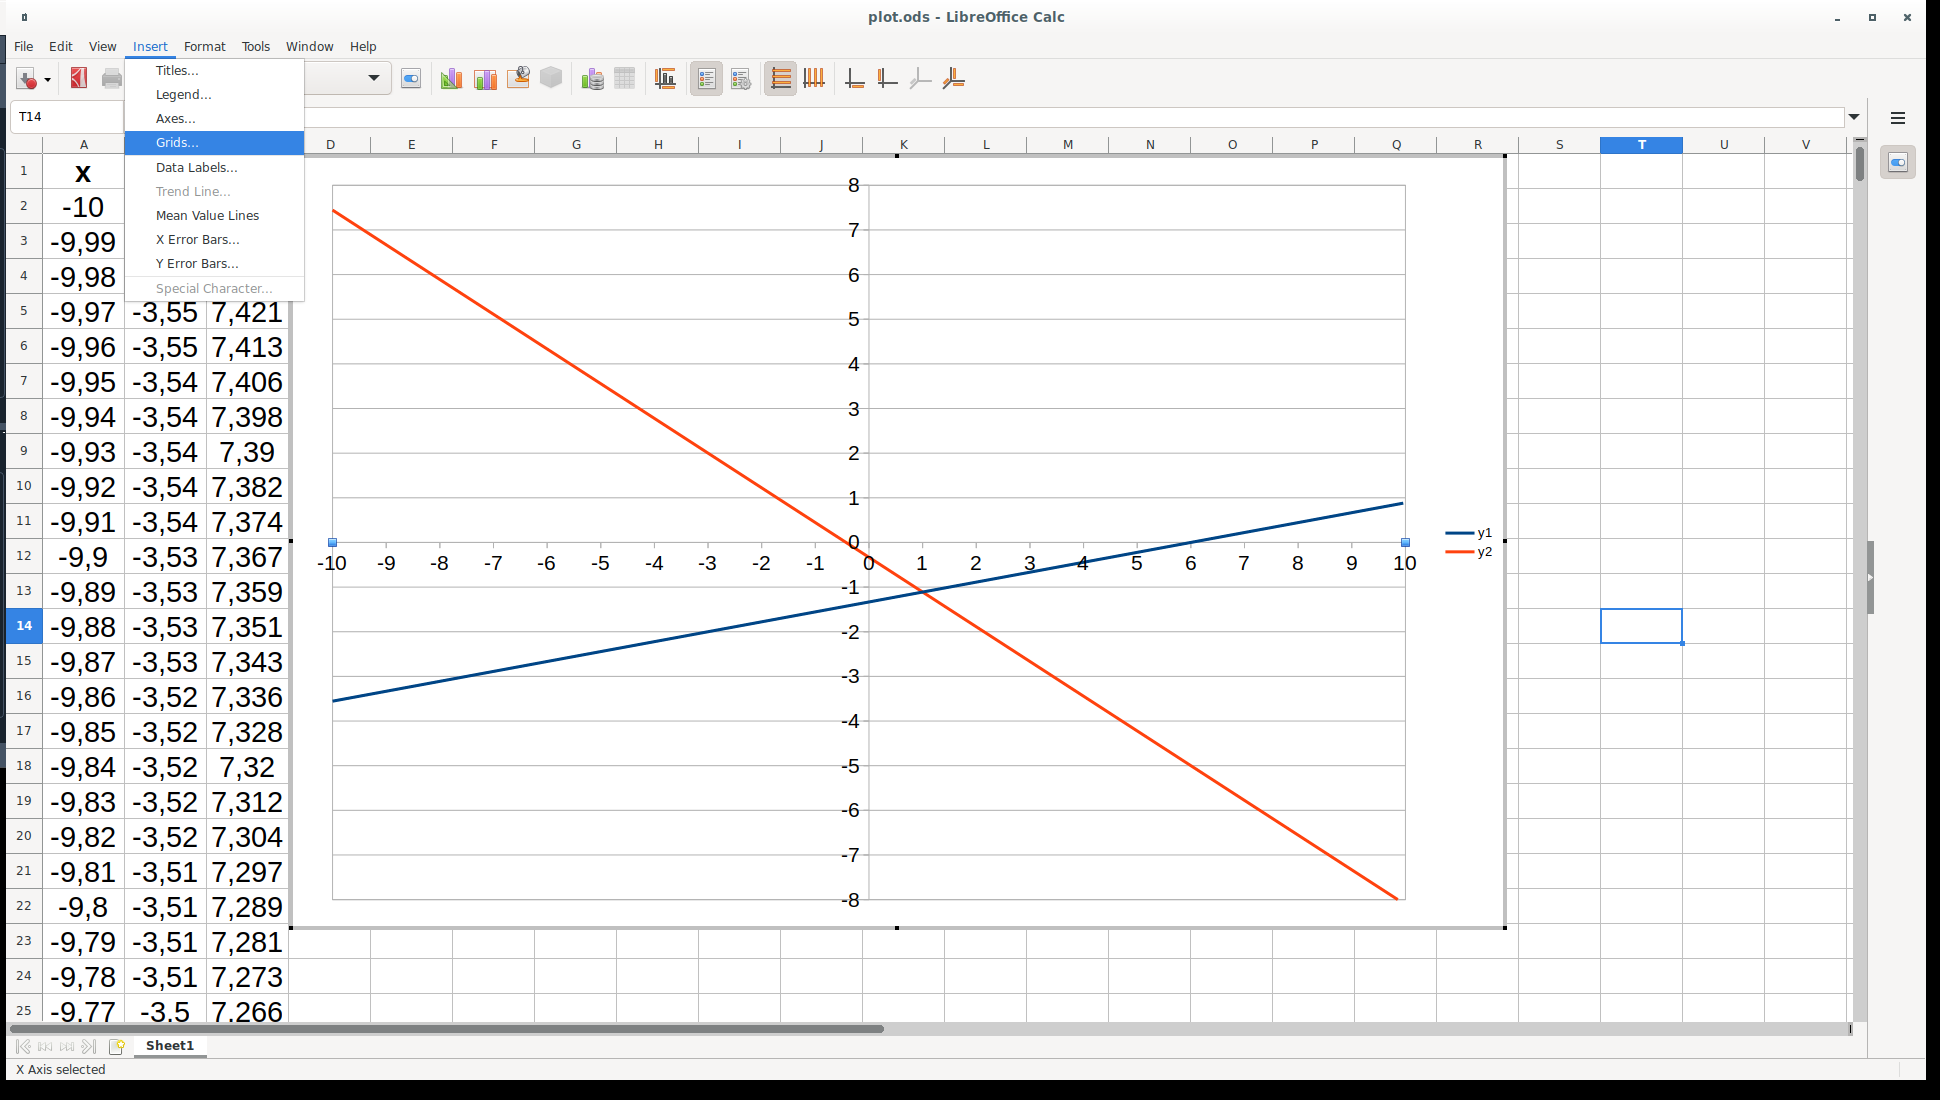
\includegraphics[width=8.0in]{pictures/picture_024.png}
  	\caption{LibreOffice Calc}
   	\label{fig:LibreOfficeCalc024}
\end{figure}
\pict{024}


%\begin{figure}[h!]		
	\centering
   	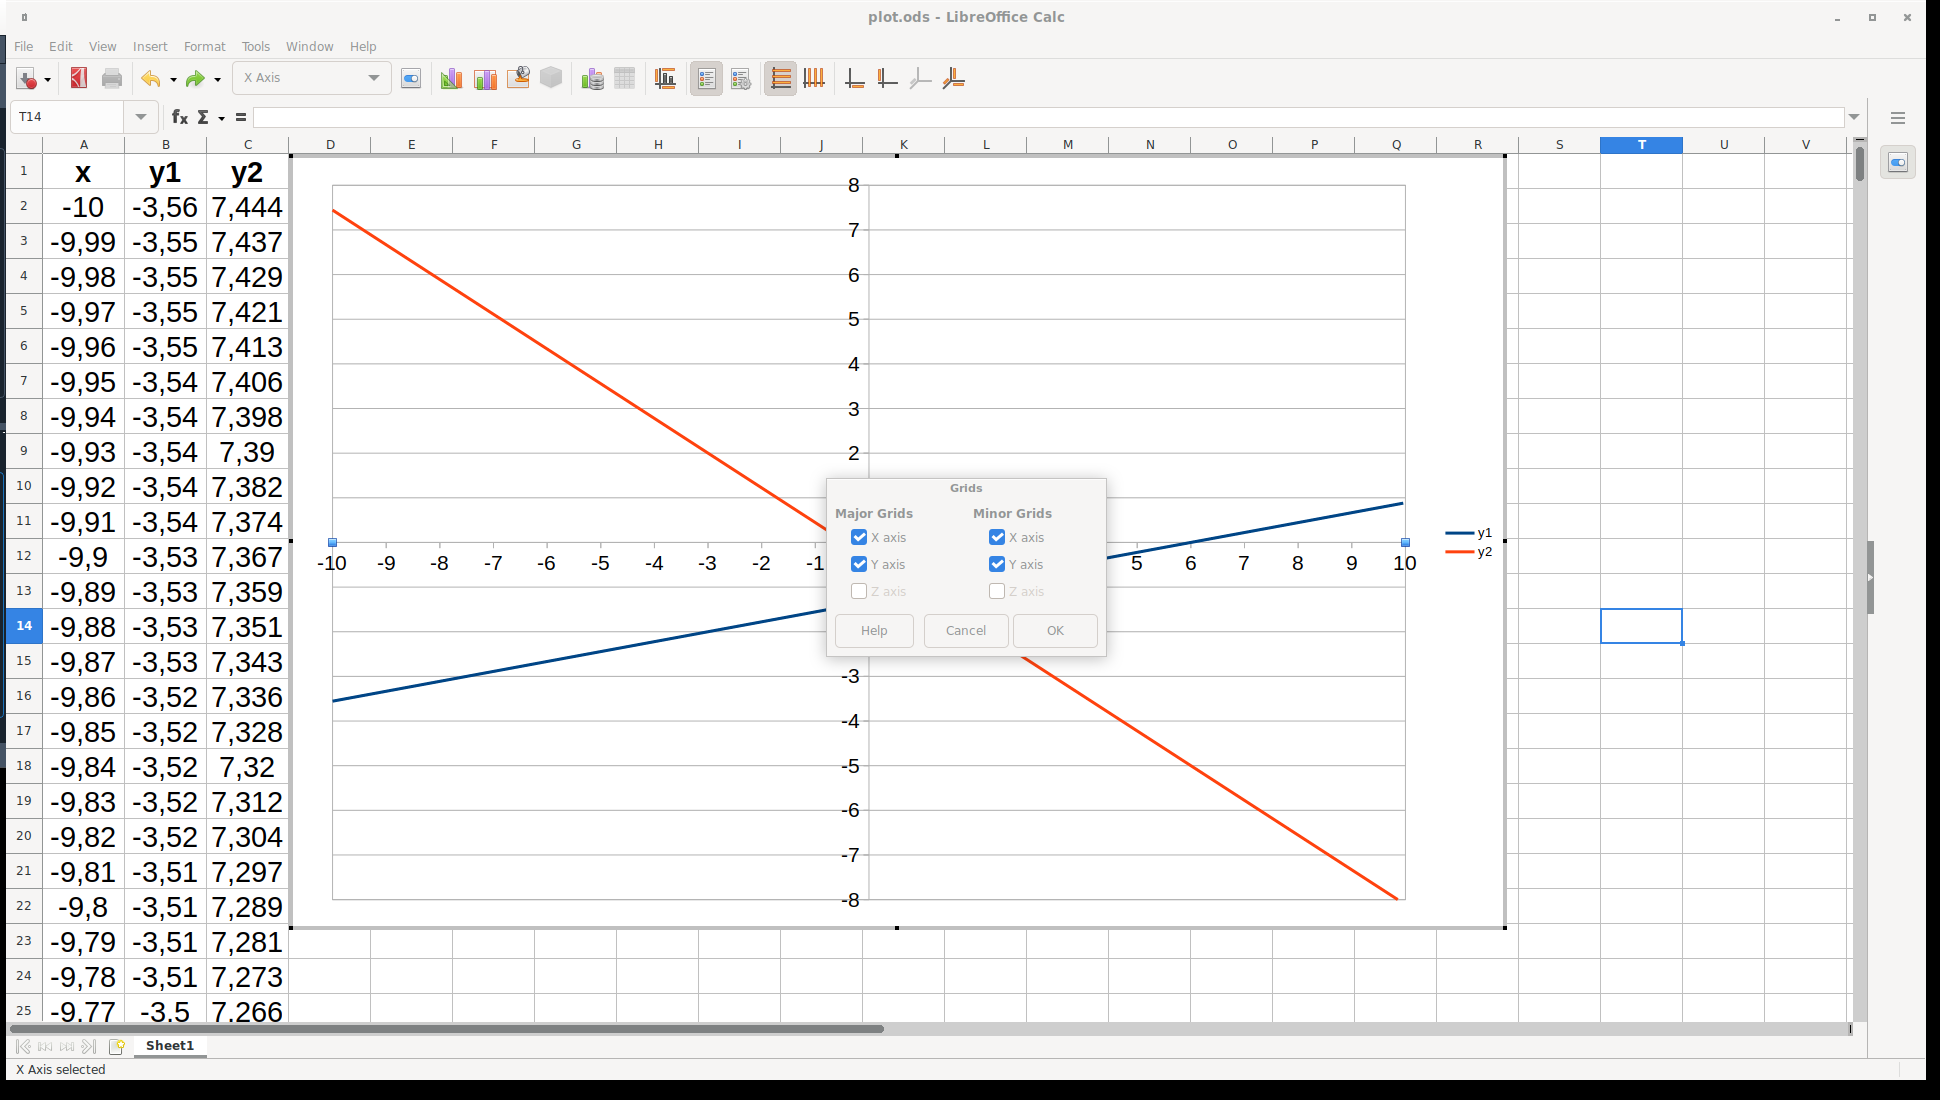
\includegraphics[width=8.0in]{pictures/picture_025.png}
  	\caption{LibreOffice Calc}
   	\label{fig:LibreOfficeCalc025}
\end{figure}
\pict{025}


%\begin{figure}[h!]		
	\centering
   	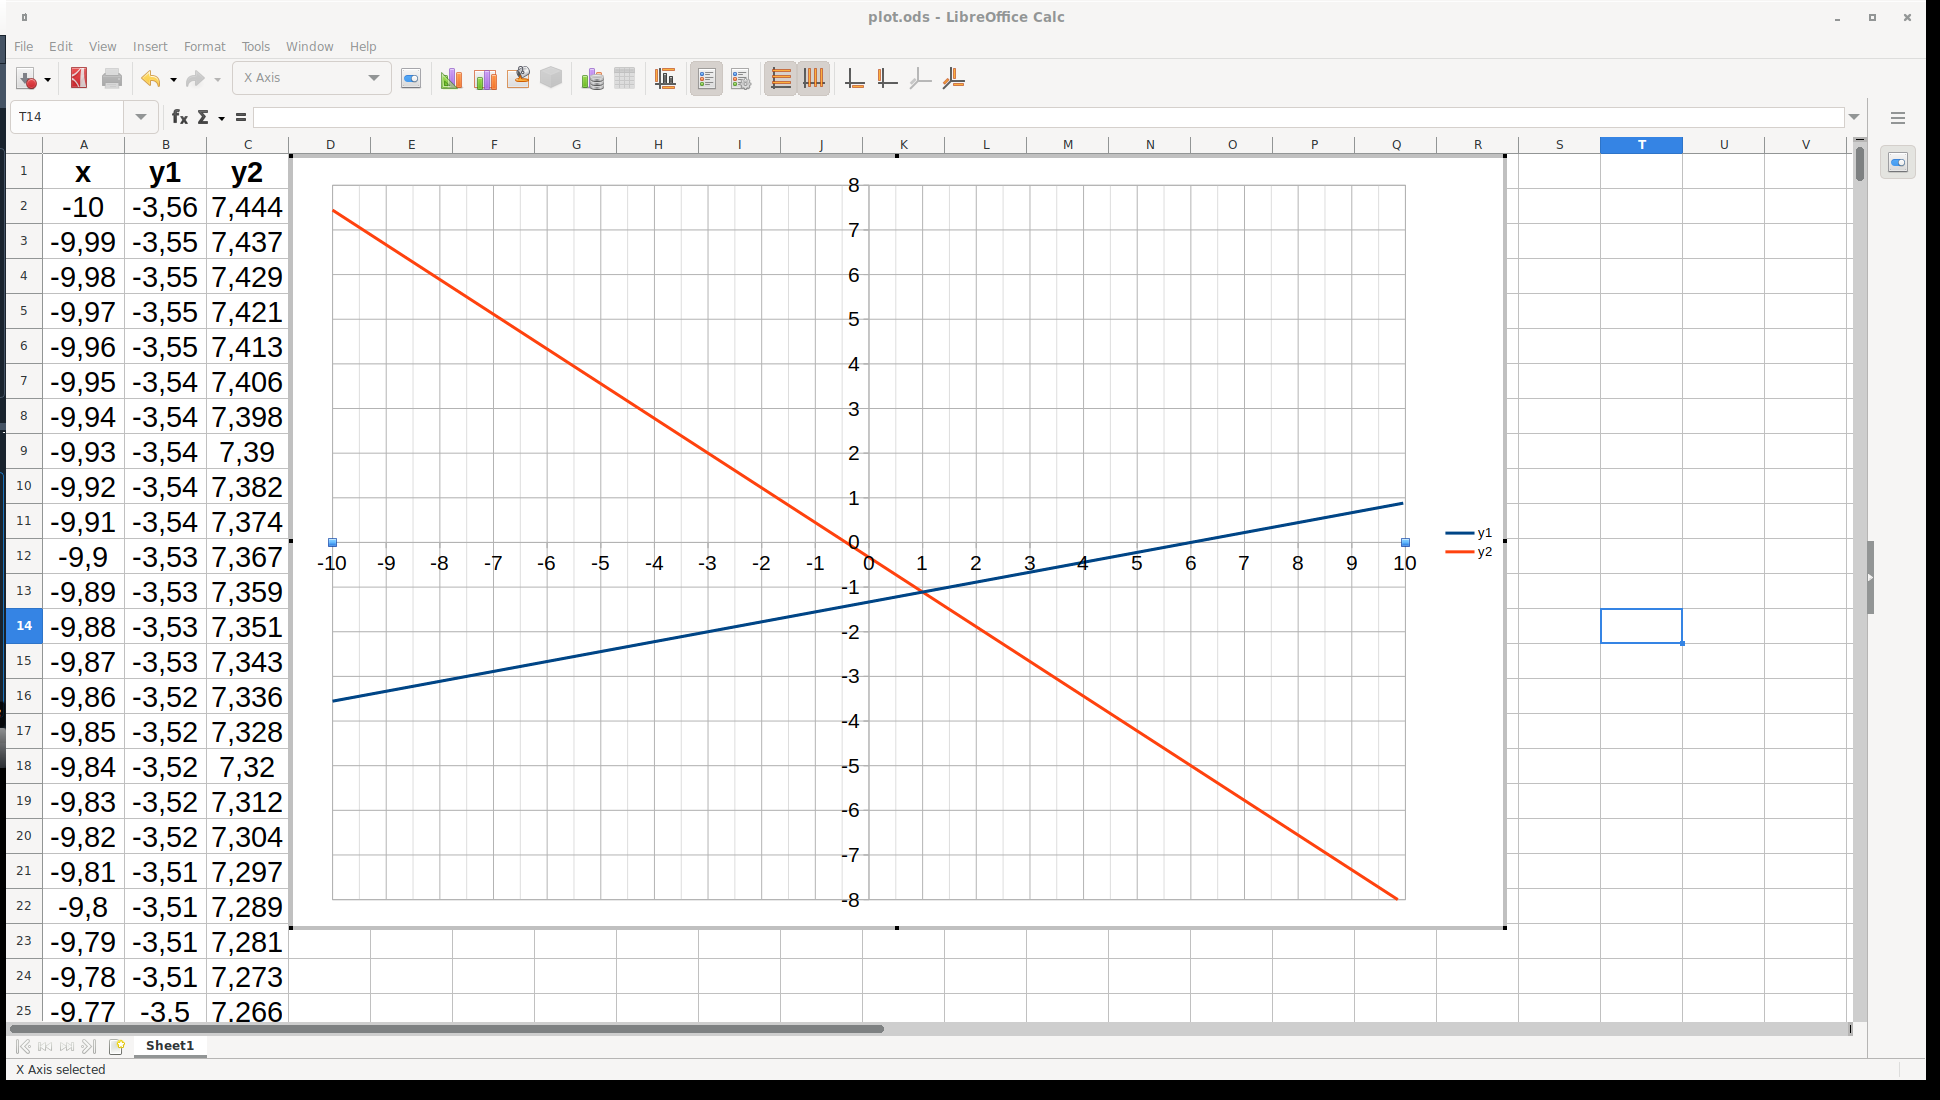
\includegraphics[width=8.0in]{pictures/picture_026.png}
  	\caption{LibreOffice Calc}
   	\label{fig:LibreOfficeCalc026}
\end{figure}
\pict{026}


%\begin{figure}[h!]		
	\centering
   	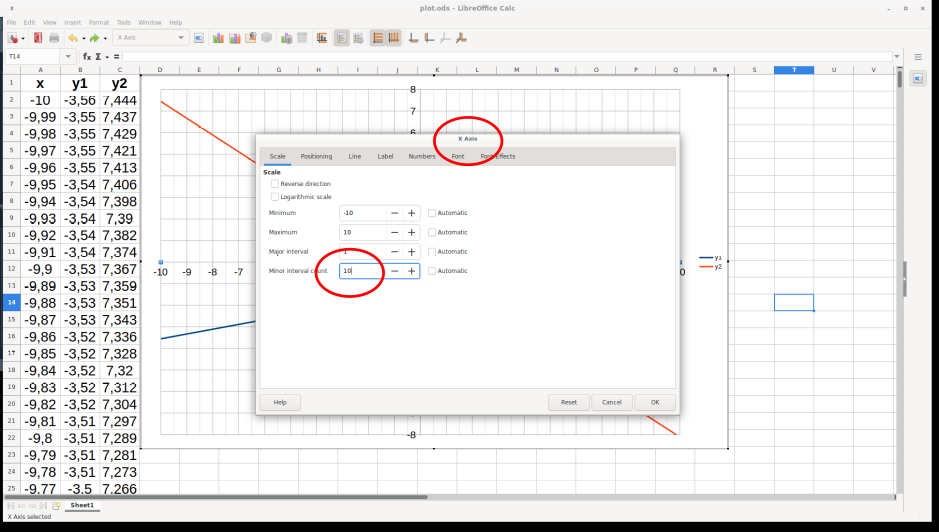
\includegraphics[width=8.0in]{pictures/picture_027.png}
  	\caption{LibreOffice Calc}
   	\label{fig:LibreOfficeCalc027}
\end{figure}
\pict{027}






%\newpage
%\mbox{}
%\newpage

\section{Infittire la griglia verticale}



%\begin{figure}[h!]		
	\centering
   	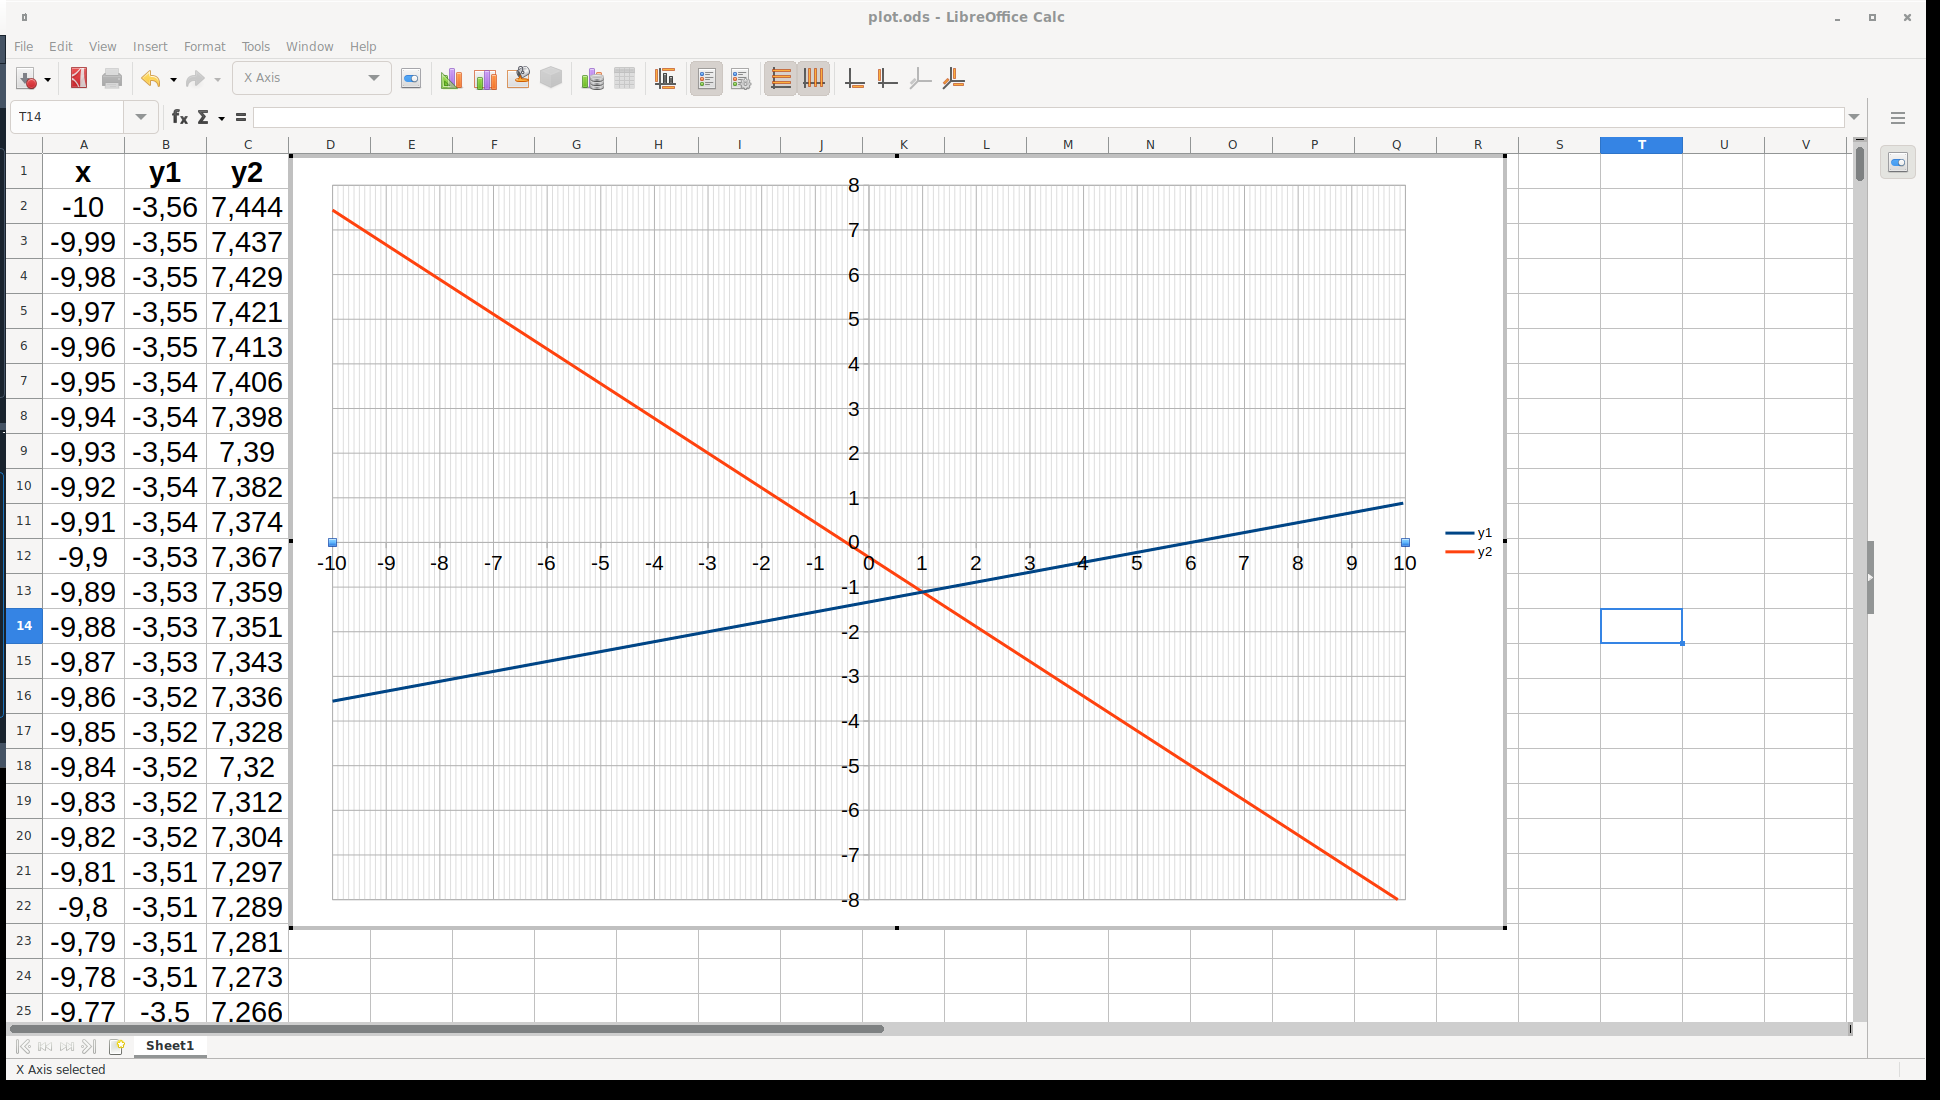
\includegraphics[width=8.0in]{pictures/picture_028.png}
  	\caption{LibreOffice Calc}
   	\label{fig:LibreOfficeCalc028}
\end{figure}
\pict{028}

\newpage


\section{Infittire la griglia orizzontale}

%\begin{figure}[h!]		
	\centering
   	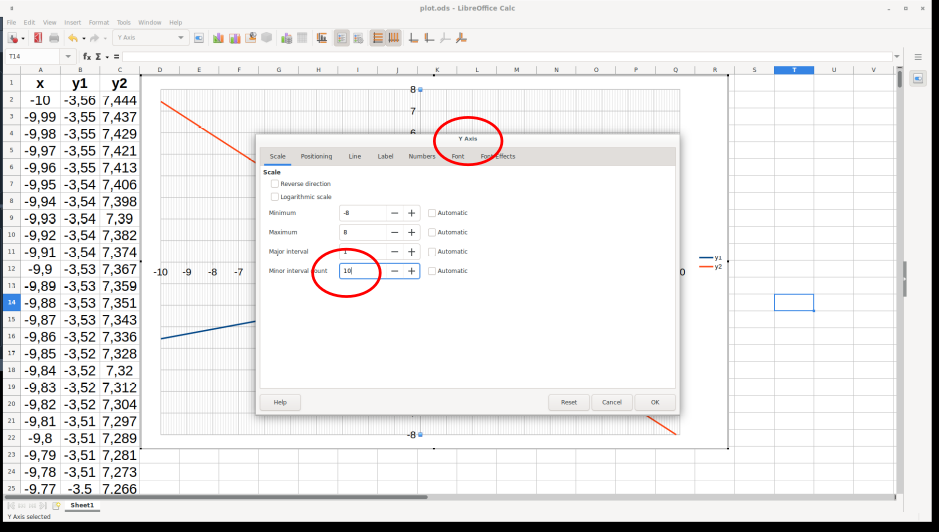
\includegraphics[width=8.0in]{pictures/picture_029.png}
  	\caption{LibreOffice Calc}
   	\label{fig:LibreOfficeCalc029}
\end{figure}
\pict{029}


%\begin{figure}[h!]		
	\centering
   	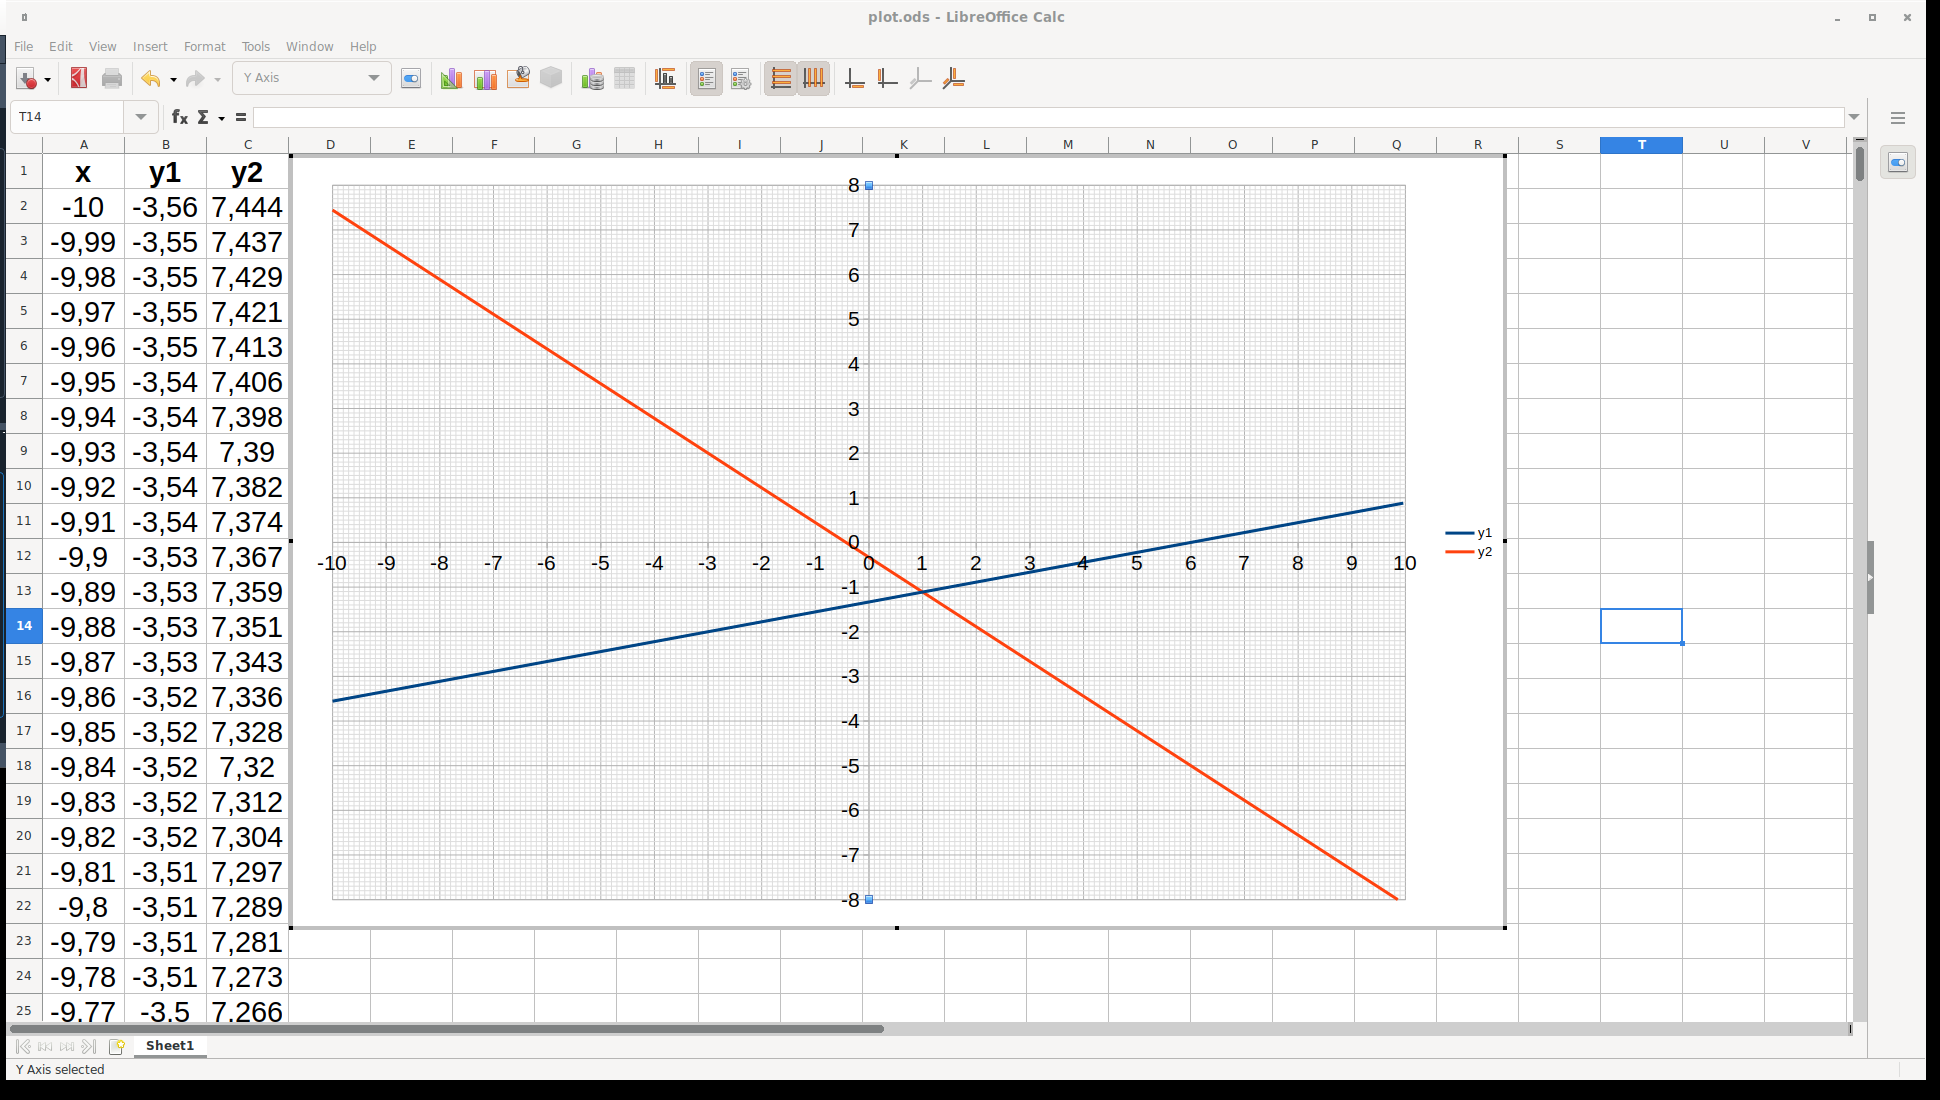
\includegraphics[width=8.0in]{pictures/picture_030.png}
  	\caption{LibreOffice Calc}
   	\label{fig:LibreOfficeCalc030}
\end{figure}
\pict{030}

\end{document}